% Sample LaTeX file for creating a paper in the Morgan Kaufmannn two
% column, 8 1/2 by 11 inch proceedings format.

\documentclass[letterpaper]{article}
\usepackage{uai2019}
\usepackage{bibli}
\usepackage[margin=1in]{geometry}

% Set the typeface to Times Roman
\usepackage{times}

\usepackage{soul}
\usepackage{url}
\usepackage[hidelinks]{hyperref}
\usepackage[utf8]{inputenc}
\usepackage[small]{caption}
\usepackage{graphicx}
\usepackage{amsmath}
\usepackage{booktabs}
\usepackage{algorithm}
\usepackage{algorithmic}
\usepackage{amsthm}
\usepackage{amssymb}
\usepackage{tikz}
\usepackage{amsfonts}
\usepackage{forloop}
\usepackage{graphicx}
\usepackage{multirow}
\usepackage{dsfont}
\usepackage{xcolor}
\usepackage{verbatim}
\usepackage{subfigure}
\usepackage[page]{appendix}

\usetikzlibrary{arrows}
\usetikzlibrary{arrows.meta}
\usetikzlibrary{decorations.markings}
\usetikzlibrary{decorations.pathreplacing}

\title{A Tighter Analysis of Randomised Policy Iteration}

\author{ {\bf Meet Taraviya} {\normalfont and} {\bf Shivaram Kalyanakrishnan} \\
Department of Computer Science and Engineering\\ Indian Institute of Technology Bombay\\
\{mtaraviya,  shivaram\}@cse.iitb.ac.in \\
}

\newtheorem{theorem}{Theorem}
\newtheorem{lemma}[theorem]{Lemma}
\newtheorem{corollary}[theorem]{Corollary}
\newtheorem{definition}[theorem]{Definition}

\newcommand{\floor}[1]{\lfloor{#1}\rfloor}
\newcommand{\ceil}[1]{\lceil{#1}\rceil}
\newcommand{\highlight}[1]{\textcolor{red}{#1}}

\begin{document}

\maketitle

\begin{abstract}
\vspace{-5pt}
Policy Iteration (PI) is a popular family of algorithms to compute an optimal policy for a given Markov Decision Problem (MDP). Starting from an arbitrary initial policy, PI repeatedly performs locally-improving switches until an optimal policy is found. The exact form of the switching rule gives rise to different variants of PI. Two decades ago, Mansour and Singh ~\shortcite{Mansour+Singh:1999} provided the first non-trivial ``strong'' upper bound on the number of iterations taken by ``Howard’s PI’’ (HPI), a widely-used variant of PI (strong bounds depend only on the number of states and actions in the MDP). They also proposed a randomised variant (RPI) and showed an even tighter strong upper bound. Their bounds for HPI and RPI have not been improved subsequently.


We revisit the algorithms and analysis of Mansour and Singh~\shortcite{Mansour+Singh:1999}. We prove a novel result on the structure of the policy space
for $k$-action MDPs, $k \geq 2$, which generalises a result known for $k = 2$. Also proposing a new counting argument, we obtain a strong bound of $(O(\sqrt{k \log k }))^{n}$ iterations for an algorithm akin to RPI, improving significantly upon Mansour and Singh's original bound of roughly $O((k/2)^{n})$. Similar analysis of a randomised variant of HPI also yields a strong upper bound of $(O(\sqrt{k \log k }))^{n}$ iterations, registering the first exponential improvement for HPI over the trivial bound of $k^{n}$. Our other contributions include a lower bound of $\Omega(n)$ iterations for RPI and an upper bound of $1.6001^{n}$ iterations for a randomised variant of ``Batch-Switching PI''~\cite{Kalyanakrishnan+MG-bspi:2016} on $2$-action MDPs---the tightest strong upper bound shown yet for the PI family.
\end{abstract}

\section{INTRODUCTION}
\label{sec:introduction}

Markov Decision Problems (MDPs)~\cite{Bellman:1957,Puterman:1994} are an abstraction of sequential decision making, providing a formal basis for problems such as automated planning and reinforcement learning. Applications of MDPs span a variety of domains~\cite{White:1985,White:1988,Feinberg+Schwarz:2002}.

An MDP describes an agent's \textit{environment}. For each state $s \in S$ in which the agent can be, and for each action $a \in A$ that it can take, the MDP specifies for all $s^{\prime} \in S$ the probability that taking $a$ from $s$ will reach $s^{\prime}$. Denote this probability$ P(s, a, s^{\prime})$. The transition from $s$ to $s^{\prime}$ by taking action $a$ also yields a numeric reward $R(s, a, s^{\prime})$. %\highlight{Here, $S$ and $A$ are finite sets.}

The agent's behaviour is encoded as a \textit{policy} $\pi: S \to A$, which specifies the action $\pi(s)$ that the agent must take from each state $s \in S$. If indeed the agent starts from some state $s^{0} \in S$ and follows $\pi$, then it encounters a random ``state-reward'' sequence $s^{0}, r^{0}, s^{1}, r^{1}, \dots$ over time, wherein for $t \geq 0$, $s^{t + 1}$ is drawn according to $P(s^{t}, \pi(s^{t}), \cdot)$, and $r^{t} = R(s^{t}, \pi(s^{t}), s^{t + 1})$. The \textit{value} of $s^{0}$ is commonly defined to be $\mathbb{E}[r^{0} + \gamma r^{1} + \gamma^{2} r^{2} + \dots]$, where $\gamma \in [0, 1)$ is a discount factor. An MDP is fully specified by $S$, $A$, $P$, $R$, and $\gamma$. In this paper, we shall assume that $S$ and $A$ are both finite.

Our definition above interprets value as ``infinite discounted reward''. The analysis provided in our paper can also be applied if alternative definitions such as ``average reward''~\cite{Mahadevan:1996}
and ``total reward''~\cite{Fearnley:2010} are used. Also, it suffices for our purposes to consider policies that do not vary over time, and which map states to actions (rather than map histories to distributions over actions). In other words, we consider policies that are stationary, deterministic, and Markovian.

%\highlight{\footnote{\highlight{We only consider stationary deterministic Markovian policies}}} 


Let $(S, A, P, R, \gamma)$ be an arbitrary MDP, and $\Pi$ be the set of all policies for this MDP. It is a well-known result that there is an \textit{optimal policy} $\pi^{\star} \in \Pi$ such that for all $\pi \in \Pi$, $s \in S$, $V^{\pi^{\star}}(s) \geq V^{\pi}(s)$. The problem we consider in this paper is precisely that of computing an optimal policy for a given MDP. We assume that $P$ and $R$ are provided as tables; there is no need for sampling (as is typical in reinforcement learning~\cite{Sutton+Barto:1998}) or for any sort of generalisation (as is needed when $S$ or $A$ are very large~\cite{Bertsekas+Tsitsiklis:1996}). Over the decades, many families of algorithms have been proposed to solve
the problem we consider, which is denoted MDP planning. Approaches vary from formulations using Linear Programming to dynamic programming techniques such as Value Iteration, Policy Iteration, and combinations~\cite{Littman+DK:1995}.

In this paper, we consider the Policy Iteration (PI) family of algorithms~\cite{Howard:1960}. PI is a conceptually-simple, iterative approach to search the space of policies. Although experimenters tend to find PI to work very well in practice~\cite[see Section 4.2]{Littman+DK:1995}, there has only been limited progress towards formally quantifying its running time. We restrict our focus to \textit{strong} running-time bounds---those that depend only on the number of states and actions in the given MDP. Strong bounds have long held appeal from a theoretical standpoint~\cite{Megiddo:1982}. Suppose we assume that arithmetic, relational and logical operations can all be performed exactly, in constant time, regardless of the operand size, the question is how many operations are needed to compute an optimal policy. The number of operations performed by PI is known to be polynomial in the number of states and actions if associated parameters such as the discount rate $\gamma$ and the number of bits $B$ needed to represent the MDP are treated as constants~\cite{Ye:2011,Scherrer:2013}. Strong bounds, on the other hand, have no dependence on parameters such as $\gamma$ and $B$.

The first non-trivial strong bounds for PI were provided by Mansour and Singh~\shortcite{Mansour+Singh:1999}, who showed an improved upper bound on the running time of Howard's PI (a commonly-used variant), and proposed a randomised variant of PI with a tighter upper bound. More recently, even tighter strong upper bounds have been shown for newer variants of PI---both deterministic~\cite{Kalyanakrishnan+Gupta} and randomised~\cite{Kalyanakrishnan+MG:2016}.

Our main contributions are based on the algorithms and analysis of Mansour and Singh~\shortcite{Mansour+Singh:1999}. Applying some fresh ideas in conjunction with their proof structure, we show significantly tighter upper bounds for related randomised algorithms, including a variant of Howard's PI, on $k$-action MDPs, $k \geq 3$. We provide a \textit{lower} bound for the randomised variant of Mansour and Singh~\shortcite{Mansour+Singh:1999}, matching a bound shown previously for Howard's PI. We also investigate a randomised ``batch-switching'' variant of PI~\cite{Kalyanakrishnan+MG-bspi:2016}. While the (strong) upper bound we furnish for this variant is the tightest yet for the PI family, experiments suggest that the randomised algorithm of Mansour and Singh~\shortcite{Mansour+Singh:1999} might itself be more efficient.

We present our technical contributions in sections \ref{sec:upperbounds} and \ref{sec:lowerbound}, after first describing PI in Section~\ref{sec:policy_iteration} and surveying previous analyses in Section~\ref{sec:relatedworkandcontribution}. In Section~\ref{sec:experiments} we share experimental findings to accompany our theoretical results. We conclude with a discussion in Section~\ref{sec:conclusion}.




\section{POLICY ITERATION}
\label{sec:policy_iteration}

In this section, we formalise Policy Iteration (PI), borrowing notation and definitions from Mansour and Singh~\shortcite{Mansour+Singh:1999}. We assume that the set of states $S$ and the set of actions $A$ are finite, with $|S| = n \geq 1$ and $|A| = k \geq 2$. Specifically, we take $A = \{0, 1, \dots, k - 1\}$.

\textit{Policy evaluation} is a basic step that is used in PI and many other approaches for MDP planning. Given a policy $\pi \in \Pi$, observe that state values (together the \textit{value function} $V^{\pi}$) satisfy a recursive relation: for $s \in S$,  $$V^{\pi}(s) = \sum_{s^{\prime} \in S} P(s, \pi(s), s^{\prime}) (R(s, \pi(s), s^{\prime}) + \gamma V^{\pi}(s^{\prime})).$$ Hence, a given policy $\pi$ can be \textit{evaluated} (that is, $V^{\pi}$ computed) by solving a system of linear equations.

For policies $\pi, \pi^{\prime} \in \Pi$, we write $\pi \succeq \pi^{\prime}$ if for all $s \in S$, $V^{\pi}(s) \geq V^{\pi^{\prime}}(s).$ If $\pi \succeq \pi^{\prime}$, and in addition, for some $s \in S$, $V^{\pi}(s) > V^{\pi^{\prime}}(s)$, then we write $\pi \succ \pi^{\prime}$. Observe that if $\pi \succeq \pi^{\prime}$ and $\pi^{\prime} \succeq \pi$, then $V^{\pi}$ and $V^{\pi^{\prime}}$ must be equal, in which case we write $\pi \approx \pi^{\prime}$. We find it convenient to distinguish between such ``equally-good'' policies by using an arbitrary total order $L$ on $\Pi$. Since policies can be represented as $n$-length $k$-ary strings from $\{0, 1, \dots, k - 1\}^{n}$, we take that for $\pi, \pi^{\prime} \in \Pi$, $\pi L \pi^{\prime}$ if and only if $\pi$ lexicographically precedes or equals $\pi^{\prime}$. We define $\pi \gtrsim \pi^{\prime}$ if (1) $\pi \succ \pi^{\prime}$ or (2) $\pi \approx \pi^{\prime}$ and $\pi L \pi^{\prime}$. By this definition, observe that there is a \textit{unique} optimal policy $\pi^{\star}$ such that for all $\pi \in \Pi$, $\pi^{\star} \gtrsim \pi$. Our algorithms will be designed to find this policy.

A na\"{i}ve way to find $\pi^{\star}$ would be to evaluate each of the $k^{n}$ policies in $\Pi$ and then compare them. As we see next, the PI family of algorithms exploits an interesting structure of the policy space to find $\pi^{\star}$ more efficiently.

The \textit{action value function} $Q^{\pi}$ for a policy $\pi \in \Pi$ provides for each $s \in S$, $a \in A$ the expected long-term reward obtained by taking $a$ from $s$ for a single time step, and thereafter acting according to $\pi$. It follows that $$Q^{\pi}(s, a) = \sum_{s^{\prime} \in S} P(s, a, s^{\prime}) (R(s, a, s^{\prime}) + \gamma V^{\pi}(s^{\prime})).$$ Now, define $T^\pi$ as follows:
\begin{align*}
T^\pi =& \{(s,a) | Q^\pi(s,a) > V^\pi(s)\} \cup\\
& \{(s, a) | Q^\pi(s,a) = V^\pi(s) \text{ and } a < \pi(s)\}.
\end{align*}
If $(s, a) \in T^{\pi}$, then $s$ is termed an ``improvable state'' for $\pi$ and $a$ an ``improving action'' at $s$ for $\pi$. For fixed $\pi$, let $\textsf{states}(T^{\pi})$ denote the set of all improvable states $s \in S$, and $T^{\pi}(s)$ denote the set of all improving actions for fixed $s \in S$,  with the convention that $T^{\pi}(s) = \emptyset$ if $s \notin \textsf{states}(T^{\pi})$. Now, if $|T^{\pi}| > 0$, let $U \subseteq T^{\pi}$ be such that $|U| \geq 1$, and no two distinct elements $(s, a)$ and $(s^{\prime}, a^{\prime}) \in U$ have $s = s^{\prime}$. In other words, $U$ collects a subset of improvable states---denoted $\textsf{states}(U)$---and exactly one improving action for each such state. In general, there can be many choices of $U$ that satisfy this property for $T^{\pi}$. For some fixed $U$, let $\textsf{modify}(\pi, U)$ denote the policy $\pi^{\prime}$ such that for all $(s, a) \in U$, $\pi^{\prime}(s) = a$ and for all $s \in S \setminus \textsf{states}(U)$, $\pi^{\prime}(s) = \pi(s)$. We collect all such policies $\pi^{\prime}$, each derived from a different choice of $U$, in a set $I(\pi)$: the set of (locally) ``improving'' policies of $\pi$. Observe that $|I(\pi)| = \prod_{s \in S} (|T^{\pi}(s)| + 1) - 1,$
and so $I(\pi)$ is empty if and only if $T^{\pi}$ is empty. The Policy Improvement Theorem, provided below, is a well-known result highlighting the relevance of $I(\pi)$. We omit the proof, which is provided by several other sources~\cite{Szepesvari:2010,Bertsekas:2012,Kalyanakrishnan+MG:2016}.
\begin{theorem}
\label{thm:pi}
For $\pi \in \Pi$: (1) if $T^{\pi} = \emptyset$, then for all $\pi^{\prime} \in \Pi$, $\pi \gtrsim \pi^{\prime}$; (2) else for all $\pi^{\prime} \in I(\pi)$, $\pi^{\prime} \gtrsim \pi$.
\end{theorem}
The theorem allows us to test if a given policy $\pi$ is optimal, and if it is not, to update to a dominating policy $\pi^{\prime}$. The PI family of algorithms is based on repeatedly performing such updates until eventually, an optimal policy is reached. Given $\pi \in \Pi$, observe that $V^{\pi}$ and $Q^{\pi}$, and therefore $T^{\pi}$, can be computed efficiently---using $\text{poly}(n, k)$ arithmetic and comparison operations. The complexity of PI is therefore determined primarily by the number of iterations performed to reach $\pi^{\star}$. Algorithms in the PI family are set apart by their ``switching rules'': how they pick $U \subseteq T^{\pi}$  for setting $\pi^{\prime} = \textsf{modify}(\pi, U)$. In general, these algorithms can be randomised. We discuss several PI variants in the next section, but before proceeding, present two related ideas.

First, it is convenient for our analysis to also consider the ``opposite'' of policy-improvement: only switching to actions that are \textit{not} improving. The following corollary is easily proven in the same manner as Theorem~\ref{thm:pi}.

\begin{corollary}
\label{cor:pd}%Policy "deprovement"
For $\pi, \pi^{\prime} \in \Pi$, suppose for all $s \in S: (\pi^{\prime}(s) \neq \pi(s)) \implies (\pi^{\prime}(s) \notin T^{\pi}(s))$. Then $\pi \gtrsim \pi^{\prime}$.
\end{corollary}

Second, it is worth noting that while our primary focus is the application of PI to MDPs, the upper bounds we show in Section~\ref{sec:upperbounds}, and indeed those originally given by Mansour and Singh~\shortcite{Mansour+Singh:1999}, also hold for solving a class of discrete objects called Acyclic Unique Sink Orientations (AUSOs)~\cite{Stickney+Watson:1978,Szabo+Welzl:2001}. Now, it follows from Theorem~\ref{thm:pi} and Corollary~\ref{cor:pd} that any two policies $\pi$ and $\pi^{\prime}$ that differ in exactly one state must satisfy either $\pi \gtrsim \pi^{\prime}$ or $\pi^{\prime} \gtrsim \pi$. Thus, in particular, policies for 2-state MDPs can be arranged as vertices of an $n$-dimensional hypercube, with edges (1) connecting policies that 
differ in exactly one state, and (2) oriented according to $\gtrsim$. Each face of the hypercube is guaranteed to have a unique sink and no cycles, making the hypercube an AUSO~\cite{Kalyanakrishnan+Gupta}. Figures \ref{fig:example-mdp}--\ref{fig:example-auso} illustrate the relationship between $2$-action MDPs and AUSOs with an example.

\begin{figure}[b!]
\centering   %%% not \center
\subfigure[]{
\label{fig:example-mdp}
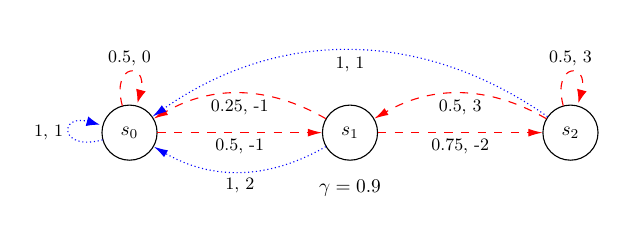
\begin{tikzpicture}[node distance=3cm,auto,scale=0.7,transform shape,
-{Latex[length=1.8mm,width=1mm]},>=Latex]

  % \begin{tikzpicture}[node distance=3cm,auto,scale=0.6, every node/.style={scale=0.6},->]
    % \tikzstyle{state}=[circle,draw=black,minimum size=13mm]
    % \tikzstyle{sink}=[draw=black,minimum size=12mm]
    \tikzset{state/.style={circle,draw=black,minimum size=10mm}}

    \node[state] at (-2, 0) (s0){$s_0$};
    \node[state] at (2, 0)(s1){$s_1$};
    \node[state] at (6, 0)(s2){$s_2$};
    % \node[state] at (0, -3.464)(s2){$s_2$};
    \node at (2, -1) {$\gamma = 0.9$};

    \draw(s0) edge [dashed, red, loop above] node {\small\textcolor{black}{0.5, 0}}  (s0);
    \draw(s0) edge [dashed, red] node[below] {\small\textcolor{black}{0.5, -1}}  (s1);
    \draw(s1) edge [dashed, red, bend right=30] node {\small\textcolor{black}{0.25, -1}}  (s0);
    \draw(s1) edge [dashed, red] node[below] {\small\textcolor{black}{0.75, -2}}  (s2);
    \draw(s2) edge [dashed, red, bend right=30] node {\small\textcolor{black}{0.5, 3}}  (s1);
    \draw(s2) edge [dashed, red, loop above] node {\small\textcolor{black}{0.5, 3}}  (s2);

    \draw(s0) edge [densely dotted, blue, loop left] node {\small\textcolor{black}{1, 1}}  (s0);
    \draw(s1) edge [densely dotted, blue, bend left=30] node {\small\textcolor{black}{1, 2}}  (s0);
    \draw(s2) edge [densely dotted, blue, bend right=35] node {\small\textcolor{black}{1, 1}}  (s0);

    \normalsize

  \end{tikzpicture}
}
\subfigure[]{
\label{tab:evaluations}

% \begin{table}[b]
\footnotesize
\setlength\tabcolsep{1.9pt}
\begin{tabular}{|c|c|c|c|c|}
\hline
$\pi$ & $V^\pi(s_0)$ & $V^\pi(s_1)$ & $V^\pi(s_2)$ & $T^\pi$ \\ \hline
000 & 4.45 & 6.55 & 10.82 & $\{(s_0, 1)\}$ \\ \hline
001 & -5.61 & -5.74 & -4.05 & $\{(s_0, 1), (s_1, 1), (s_2, 0)\}$ \\ \hline
010 & 2.76 & 4.48 & 9.12 & $\{(s_0, 1), (s_1, 0) \}$ \\ \hline
011 & 2.76 & 4.48 & 3.48 & $\{(s_0, 1), (s_2, 0)\}$ \\ \hline
100 & 10.00 & 9.34 & 13.10 & $\{(s_1, 1) \}$ \\ \hline
101 & 10.00 & 7.25 & 10.00 & $\{(s_1, 1), (s_2, 0)\}$ \\ \hline
110 & 10.00 & 11.00 & 14.45 & $\{\}$ \\ \hline
111 & 10.00 & 11.00 & 10.00 & $\{(s_2, 0)\}$ \\ \hline
% \textcolor{red}{0}\textcolor{red}{0}\textcolor{red}{0} & 4.45 & 6.55 & 10.82 & $\{(s_0, \textcolor{blue}{1})\}$ \\ \hline
% \textcolor{red}{0}\textcolor{red}{0}\textcolor{blue}{1} & -5.61 & -5.74 & -4.05 & $\{(s_0, \textcolor{blue}{1}), (s_1, \textcolor{blue}{1}), (s_2, \textcolor{red}{0})\}$ \\ \hline
% \textcolor{red}{0}\textcolor{blue}{1}\textcolor{red}{0} & 2.76 & 4.48 & 9.12 & $\{(s_0, \textcolor{blue}{1}), (s_1, \textcolor{red}{0})\}$ \\ \hline
% \textcolor{red}{0}\textcolor{blue}{1}\textcolor{blue}{1} & 2.76 & 4.48 & 3.48 & $\{(s_0, \textcolor{blue}{1}), (s_2, \textcolor{red}{0})\}$ \\ \hline
% \textcolor{blue}{1}\textcolor{red}{0}\textcolor{red}{0} & 10.00 & 9.34 & 13.10 & $\{(s_1, \textcolor{blue}{1})\}$ \\ \hline
% \textcolor{blue}{1}\textcolor{red}{0}\textcolor{blue}{1} & 10.00 & 7.25 & 10.00 & $\{(s_1, \textcolor{blue}{1}), (s_2, \textcolor{red}{0})\}$ \\ \hline
% \textcolor{blue}{1}\textcolor{blue}{1}\textcolor{red}{0} & 10.00 & 11.00 & 14.45 & $\{\}$ \\ \hline
% \textcolor{blue}{1}\textcolor{blue}{1}\textcolor{blue}{1} & 10.00 & 11.00 & 10.00 & $\{(s_2, \textcolor{red}{0})\}$ \\ \hline
\end{tabular}
% \end{table}
\normalsize
}
\subfigure[]{
\label{fig:example-lattice}
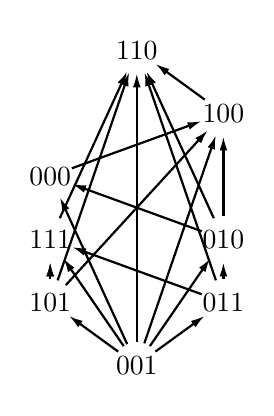
\begin{tikzpicture}[node distance=3cm,auto,scale=2,
-{Latex[length=1.8mm,width=1mm]},>=Latex]
     \tikzstyle{vertex}=[circle,minimum size=10pt,inner sep=0pt]
     \tikzstyle{edge} = [draw,thick,black]
     \node[vertex] (v0) at (-0.55, +1.2) {$000$};
     \node[vertex] (v1) at (+0.0, +0.0) {$001$};
     \node[vertex] (v2) at (+0.55, +0.8) {$010$};
     \node[vertex] (v3) at (+0.55, +0.4) {$011$};
     \node[vertex] (v4) at (+0.55, +1.6) {$100$};
     \node[vertex] (v5) at (-0.55, +0.4) {$101$};
     \node[vertex] (v6) at (+0.0, +2.0) {$110$};
     \node[vertex] (v7) at (-0.55, +0.8) {$111$};

     \draw[edge] (v0) -- (v4);
     \draw[edge] (v1) -- (v0);
     \draw[edge] (v1) -- (v3);
     \draw[edge] (v1) -- (v5);
     \draw[edge] (v2) -- (v6);
     \draw[edge] (v2) -- (v0);
     \draw[edge] (v3) -- (v7);
     \draw[edge, bend right] (v3) -- (v2);
     \draw[edge] (v4) -- (v6);
     \draw[edge] (v5) -- (v7);
     \draw[edge] (v5) -- (v4);
     \draw[edge] (v7) -- (v6);

     \draw[edge] (v2) -- (v4);
     \draw[edge, bend left] (v5) -- (v7);
     \draw[edge] (v5) -- (v6);
     \draw[edge] (v3) -- (v6);
     \draw[edge] (v1) -- (v2);
     \draw[edge] (v1) -- (v4);
     \draw[edge] (v1) -- (v6);
     \draw[edge] (v1) -- (v7);
 \end{tikzpicture}
}
\hspace{8.0pt}
\subfigure[]{
\label{fig:example-auso}
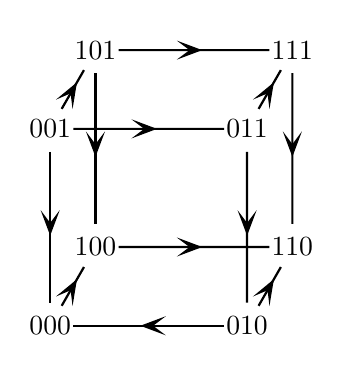
\begin{tikzpicture}[scale=2.5]
\pgfarrowsdeclare{mytipcube}{mytipcube} 
{ 
  \arrowsize=0.2pt 
  \advance\arrowsize by .5\pgflinewidth 
  \pgfarrowsleftextend{-4\arrowsize-2\pgflinewidth} 
  \pgfarrowsrightextend{2\pgflinewidth} 
} 
{ 
  \arrowsize=0.75pt 
  \advance\arrowsize by .5\pgflinewidth 
  \pgfsetdash{}{0pt} % do not dash 
  \pgfsetroundjoin   % fix join 
  \pgfsetroundcap    % fix cap 
  \pgfpathmoveto{\pgfpoint{-4\arrowsize}{3\arrowsize}}
  \pgfpathlineto{\pgfpoint{4\arrowsize}{0\arrowsize}}
  \pgfpathlineto{\pgfpoint{-4\arrowsize}{-3\arrowsize}}
  \pgfpathlineto{\pgfpoint{0\arrowsize}{0\arrowsize}}
  \pgfpathlineto{\pgfpoint{-4\arrowsize}{3\arrowsize}}
%   \pgfusepathqstroke 
  \pgfusepathqfill
}
 \tikzset{
   % style to apply some styles to each segment of a path
   on each segment/.style={
     decorate,
     decoration={
       show path construction,
       moveto code={},
       lineto code={
         \path [#1]
         (\tikzinputsegmentfirst) -- (\tikzinputsegmentlast);
       },
       curveto code={
         \path [#1] (\tikzinputsegmentfirst)
         .. controls
         (\tikzinputsegmentsupporta) and (\tikzinputsegmentsupportb)
         ..
         (\tikzinputsegmentlast);
       },
       closepath code={
         \path [#1]
         (\tikzinputsegmentfirst) -- (\tikzinputsegmentlast);
       },
     },
   },
   % style to add an arrow in the middle of a path
   mid arrow/.style={postaction={decorate,decoration={
         markings,
         mark=at position .5 with {{\arrow[#1]{mytipcube}}},
       }}},
 }

     \tikzstyle{vertex}=[circle,minimum size=0pt,inner sep=0pt]
     \tikzstyle{edge} = [draw,thick,postaction={on each segment={mid arrow=black}},black]
     \node[vertex] (v0) at (0,0) {$000$};
     \node[vertex] (v1) at (0,1) {$001$};
     \node[vertex] (v2) at (1,0) {$010$};
     \node[vertex] (v3) at (1,1) {$011$};
     \node[vertex] (v4) at (0.23, 0.4) {$100$};
     \node[vertex] (v5) at (0.23,1.4) {$101$};
     \node[vertex] (v6) at (1.23,0.4) {$110$};
     \node[vertex] (v7) at (1.23,1.4) {$111$};
    %  \node[vertex] (v0) at (0,0) {};
    %  \node[vertex] (v1) at (0,1) {};
    %  \node[vertex] (v2) at (1,0) {};
    %  \node[vertex] (v3) at (1,1) {};
    %  \node[vertex] (v4) at (0.23, 0.4) {};
    %  \node[vertex] (v5) at (0.23,1.4) {};
    %  \node[vertex] (v6) at (1.23,0.4) {};
    %  \node[vertex] (v7) at (1.23,1.4) {};

     \draw[edge] (v0) -- (v4);
     \draw[edge] (v1) -- (v0);
     \draw[edge] (v1) -- (v3);
     \draw[edge] (v1) -- (v5);
     \draw[edge] (v2) -- (v6);
     \draw[edge] (v2) -- (v0);
     \draw[edge] (v3) -- (v7);
     \draw[edge] (v3) -- (v2);
     \draw[edge] (v4) -- (v6);
     \draw[edge] (v5) -- (v7);
     \draw[edge] (v5) -- (v4);
     \draw[edge] (v7) -- (v6);
 \end{tikzpicture}
}
%\vspace{-0.5cm}
\caption{(a) Example of a $3$-state $2$-action MDP. Red (dashed) and blue (dotted) edges correspond to actions $0$ and $1$, respectively. Each arrow shows the corresponding transition probability and reward. (b) $V^\pi$ and $T^\pi$ for all $\pi\in\Pi$. (c) Graph with each policy $\pi$ as a vertex, with edges leading to all policies $\pi^{\prime} \in I(\pi)$. (d) Induced AUSO (details in text). }
\end{figure}

%For illustration, consider the $3$-state, $2$-action MDP shown in Figure~\ref{fig:example-mdp}. The table in Figure~\ref{tab:evaluations} shows the value functions of the $8$ resulting policies $\pi$, along with $T^{\pi}$. The graph in Figure~\ref{fig:example-lattice} has vertices corresponding to the $8$ policies; directed edges connect each non-optimal policy $\pi$ with all the polices in $I(\pi)$.  

%\cite{Stickney+Watson:1978}

\textit{Solving} a given AUSO amounts to identifying its sink. For so doing, an algorithm may \textit{evaluate} vertices one at a time, thereby discovering their outgoing edges. In this context, PI would begin with an arbitrary vertex $u$, and repeatedly update to some vertex $v$ in the subface formed by the outgoing edges of $u$ (thus $v$ ``locally improves'' upon $u$). If $u$ has no outgoing edges, it must be the sink.

Interestingly, it can be shown that AUSOs resulting from MDPs must additionally satisfy the \textit{Holt-Klee conditions}~\cite{Holt+Klee:1999}, which are: for an $n$-dimensional AUSO, every $d$-dimensional face, $1 \leq d \leq n$, should have at least $d$ vertex-disconnected paths from source to sink. The Holt-Klee conditions hold for all AUSOs induced by Linear Programs, and can be shown for MDPs by considering their Linear programming formulation~\cite{Post+Ye:2013}. In the example from Figure~\ref{fig:example-auso}, notice that from the source $001$, there are paths through $000$ and $100$; $011$ and $010$; and also $101$ and $111$ to the sink $110$ . All $2$- and $1$-dimensional AUSOs necessarily satisfy the Holt-Klee conditions.


\begin{comment}

and an analysis of their
Algorithms within the PI family are indeed differentiated solely by the rule they apply to pick states for switching. Most popular is Howard’s PI \cite{Howard:1960}, which implements a greedy switching rule, wherein every state in the improvable set is switched. We still have the choice on how to select the improving action for the states in the improvable set. While Mansour and Singh \shortcite{Mansour+Singh:1999} proved the upper bound for Howard's PI for an arbitrary action selection rule, we only consider a randomized rule where in we select the improving action uniformly at random from $T^\pi(s)\backslash \{\pi(s)\}$ for states in the improvable set where we have a choice of selecting the improving action. \cite{Mansour+Singh:1999} also introduced Randomized PI, wherein we select $\pi'(s)$ uniformly at random from $T^\pi(s)$ for each state $s$.

A switch corresponds to changing the actions taken by the current policy on one or more of these improvable states. Since $\forall s\in S, \pi \in \Pi: (s,\pi(s))\in T^\pi$, $|T^\pi|\ge n$. Also, for the optimal policy $\pi^{*}$, $|T^{\pi^{*}}|=n$. Formally, a switch is defined by a set $L^\pi \subseteq T^\pi$ such that $|\text{states}(L^\pi)|=|L^\pi|=n$. This condition ensures that we select only one action for each state $s\in S$. We say $\pi'$ improves upon $\pi$ if $\{(s,\pi'(s))|s\in S\}$ is a switch for $\pi$. Thus we allow $\pi'=\pi$ when $\pi$ is not optimal. Since we are only dealing with randomized algorithms, the probability of this happening is very low and it can indeed be shown that this relaxation can cause at most a constant factor difference in the bounds we will derive.

Informally, $V^\pi(s)$ is the expected return when the agent starts at states $s$ and follows $\pi$ forever, and $Q^\pi(s,a)$ is the expected return when the agent starts at state $s$, takes action $a$ and follows $\pi$ thereafter forever. For $\pi, \pi' \in \Pi$,$ s\in S$,$a,a' \in A$, we define $\gtrsim$ as
\begin{multline}
Q^\pi(s,a) \gtrsim Q^{\pi'}(s,a') \\ \hfill\null\stackrel{\text{def}}{=} Q^\pi(s,a) > Q^{\pi'}(s,a') \hfill\null\\ \hfill\null\vee (Q^\pi(s,a) = Q^{\pi'}(s,a') \wedge a \ge a')
\end{multline}
\par
Since $V^\pi(s)=Q^\pi(s,\pi(s))$, we can easily extend $\gtrsim$ to the value functions as well. We say $V^\pi \succeq V^{\pi'}$ or $\pi \succeq \pi'$ if $V^\pi(s) \gtrsim V^{\pi'}(s)$ for all $s \in S$. Using $\gtrsim$ instead of $\ge$ ensures that two unequal policies $\pi$ and $\pi'$ cannot satisfy both $\pi \succeq \pi'$ and $\pi \preceq \pi'$. Thus $(\Pi, \preceq)$ is a partial order. It is a key property, as established by Bellman \shortcite{Bellman:1957}, that this set contains a policy $\pi^{*}$ such that $\forall \pi \in \Pi$, $\pi^{*}\succeq \pi$. Such a policy is called an \textit{optimal} policy. With the modified definition where we use $\gtrsim$ instead of $\ge$, it can further be shown that there is a unique optimal policy.
% \begin{multline}
% V^\pi(s) \gtrsim V^{\pi'}(s) \\ \stackrel{\text{def}}{=} V^\pi(s) > V^{\pi'}(s) \vee (V^\pi(s) = V^{\pi'}(s) \wedge \pi(s)\ge \pi'(s))
% \end{multline}

% We say that a policy $\pi$ dominates over policy $\pi'$ \textit{at a state} $s$ or $V^\pi(s) \gtrsim V^{\pi'}(s)$ if $V^\pi(s) > V^{\pi'}(s) \vee (V^\pi(s) = V^{\pi'}(s) \wedge \pi(s)\ge \pi'(s))$. We say $\pi$ dominates over $\pi'$ if it dominates over $\pi'$ at all states. 
% \par
% Let $\Pi$ be the set of distinct policies corresponding to $M$. It is a key property, as established by Bellman \shortcite{Bellman:1957}, that this set contains a policy $\pi^{*}$ such that for $\forall s \in S$, $\pi \in \Pi$, $$V^{\pi^{*}}(s) \ge V^\pi(s)$$. Such a policy $\pi^{*}$ is called an optimal policy; in general there can be multiple optimal policies for an MDP.
\par
The problem we consider is precisely that of finding an optimal policy for a given MDP $M = (S, A, R, T, \gamma)$. Specifically, we examine the Policy Iteration (PI) family of algorithms \cite{Howard:1960}, which follow the general template of starting with some initial policy, and repeatedly performing locally improving “switches” until an optimal policy is found. Each non-optimal policy $s$ is guaranteed to have a nonempty set of “improvable” state-action pairs, which are defined as
\begin{multline}
    T^\pi \subseteq S\times A; \hfill\null\\ \hfill\null T^\pi = \{(s,a) | Q^\pi(s,a) \gtrsim V^\pi(s)\}
    \hfill\null
\end{multline}
We will use $\text{states}(T^\pi)$ to denote all the improvable states and $T^\pi(s)$ to denote all the improving actions at $s$.
\begin{multline}\hfill\null
    \text{states}(T^\pi) = \{s | \exists a: (s,a)\in T^\pi \}
    \hfill\null
\end{multline}
\begin{multline} \hfill\null
    T^\pi(s) = \{a | (s,a)\in T^\pi \}
    \hfill\null
\end{multline}
\par
A switch corresponds to changing the actions taken by the current policy on one or more of these improvable states. Since $\forall s\in S, \pi \in \Pi: (s,\pi(s))\in T^\pi$, $|T^\pi|\ge n$. Also, for the optimal policy $\pi^{*}$, $|T^{\pi^{*}}|=n$. Formally, a switch is defined by a set $L^\pi \subseteq T^\pi$ such that $|\text{states}(L^\pi)|=|L^\pi|=n$. This condition ensures that we select only one action for each state $s\in S$. We say $\pi'$ improves upon $\pi$ if $\{(s,\pi'(s))|s\in S\}$ is a switch for $\pi$. Thus we allow $\pi'=\pi$ when $\pi$ is not optimal. Since we are only dealing with randomized algorithms, the probability of this happening is very low and it can indeed be shown that this relaxation can cause at most a constant factor difference in the bounds we will derive.
\par
\end{comment}
\section{RELATED WORK}
\label{sec:relatedworkandcontribution}

%``Strong'' bounds for MDP planning are those that depend solely on the number of states and actions, and not on additional parameters such as the discount factor. \st{Although PI tends to perform extremely well in practice,} \highlight{While polynomial bounds for MDP planning with a fixed discount rate $\gamma$ are known \cite{Ye:2011},} the tightest strong bounds known for MDP planning come from Linear Programning (LP) algorithms that operate on an LP formulation of the MDP~\cite[see Section 2]{Kalyanakrishnan+Gupta}. While the bounds we have shown for RPI-UIP are exponential in $n$, it is to be noted that the LP route can yield bounds of the form $\text{poly}(n, k) \cdot \exp(O(\sqrt{n\log n}))$~\cite{Matousek+SW:1996} on the number of arithmetic operations.

In this section, we survey results on the complexity of different variants of PI. We only consider strong bounds---which solely depend on the number of states $n$ and the number of actions $k$ in the MDP. Note that polynomial upper bounds in $n$ and $k$ exist for variants of PI if dependence on additional parameters such as the discount factor $\gamma$ and the representation size $B$ are permitted~\cite{Ye:2011,Scherrer:2013}. Also note that the LP route for MDP planning can yield a strong upper bound of $\text{poly}(n, k) \cdot \exp(O(\sqrt{n
  \log n}))$~\cite{Matousek+SW:1996} operations. Strong upper bounds known yet for PI  are all exponential in $n$. Since policy evaluation is polynomial in $n$ and $k$, the bounds we discuss below are on the number of policy evaluations performed by PI.
  
We claim $u(n, k)$ as an upper bound for some variant if for \textit{every} $n$-state, $k$-action MDP, from \textit{every} starting policy, the (expected) number of policy evaluations performed is at most $u(n, k)$ (expectation needed only for randomised variants). On the other hand, $l(n, k)$ is a lower bound for some algorithm if there exist an $n$-state, $k$-action MDP and a starting policy from which the (expected) number of policy evaluations performed is at least $l(n, k)$. Table~\ref{tab:summaryofbounds} summarises existing upper bounds side-by-side with our improvements, which we proceed to present. Assume $\pi \in \Pi$ is the policy being considered for improvement and $U$ the subset of $T^{\pi}$ to be used for switching---to obtain $\pi^{\prime} = \textsf{modify}(\pi, U)$.

\begin{table}[t]
\centering
\caption{Upper bounds for PI variants for general $k$. References and descriptions of the algorithms are given in the text. Except the entry marked ``D'', all the results from this paper correspond to randomised variants, of which some are obtained by specialising or slightly altering the original variant.}
\label{tab:summaryofbounds}
\begin{tabular}{c|c|c}
\textbf{Variant} & \textbf{Previous} & \textbf{This paper}\\\hline
HPI &  $O(\frac{k^{n}}{n})$ & $(O(k \log k))^{n / 2}$\\\hline
RPI & $O(((1 + \frac{2}{\log_{2} k})\frac{k}{2})^{n})$ & $(O(k \log k))^{n / 2}$\\\hline
\multirow{2}{*}{BSPI}  & \multirow{2}{*}{$k^{0.7207n}$} & $k^{0.7019n}$ [D]\\
 &  & $k^{0.6782n}$\\\hline
RSPI & $(O(\log k))^{n}$ & --\\ \hline
\end{tabular}
\end{table}


\noindent\textbf{Howard's PI.} The earliest variant of PI, introduced by Howard~\shortcite{Howard:1960}, is also the most commonly used. Howard's PI (HPI) dictates that \textit{every} improvable state be switched; in other words, $\textit{States}(U) = \textit{States}(T^{\pi})$. For $2$-action MDPs, this description fixes the switching rule, since $|T^{\pi}(s)| \leq 1$ for every state $s$. If $k \geq 3$, there might be multiple improving actions for some state---in which case we may pick an \textit{arbitrary} one for switching. The tightest upper bound on the number of iterations taken by HPI is $O(k^{n}/n)$~\cite{Mansour+Singh:1999}; the multiplicative factor has subsequently been improved~\cite{Hollanders+GDJ:2014}. Mansour and Singh's analysis partitions $\Pi$ into a set of ``large-improvement'' policies and a set of ``small-improvement'' policies. For large-improvement policies, defined as those for which $|\textsf{states}(T^{\pi})|$ exceeds a threshold $m$, a structural argument shows that $\pi^{\prime}$ will dominate or be incomparable to at least $m$ policies that themselves dominate $\pi$. Since each large-improvement policy therefore eliminates $m$ policies, and since the number of small-improvement policies can be upper-bounded in terms of $m$, tuning $m$ yields an overall bound of $O(k^{n}/n)$ iterations.\\

\noindent\textbf{Randomised PI.} Mansour and Singh~\shortcite{Mansour+Singh:1999} also propose a randomised variant of PI (RPI), in which \textsf{states}($U$) is picked uniformly at random from  the non-empty subsets of \textsf{states}($T^{\pi}$). Again, if $k \geq 3$, improving actions can be picked arbitrarily. In this case, it can be shown that visits to large-improvement policies eliminate $\Theta(2^{m})$ policies in expectation, leading to an overall bound of $O(((1 + 2/\log_{2} k )(k/2))^{n})$ iterations. For the special case of $k = 2$, Mansour and Singh~\shortcite{Mansour+Singh:1999} provide a 
a tighter bound of $O(1.7172^{n})$ iterations.\\

\noindent\textbf{Batch-switching PI.} In a relatively recent line of work, Kalyanakrishnan et al.~\shortcite{Kalyanakrishnan+MG-bspi:2016} propose a scheme to translate upper bounds on the complexity of PI for small (constant-size) MDPs to ones for general MDPs. Arguing essentially based on the policy improvement theorem, they demonstrate that HPI can take at most $33$ iterations on $7$-state, $2$-action MDPs. This bound comes from a relaxation called the ``order regularity'' problem~ \cite{Gerencser+HDJ:2015}. Batch-switching PI (BSPI) is a variant of PI in which states only within a fixed-size batch of states are switched at each iteration. Assuming that batches are indexed, the batch with the highest index among those with improvable states is picked. For a batch size of $7$, a recursive argument establishes that BSPI can take at most $33^{n/7} < 1.6479^{n}$ iterations on $2$-action MDPs. The numerical computation of the bound for batch sizes $8$ and higher has not been feasible, although evidence suggests that larger batch sizes might be even more economical. If such a trend is indeed true, then HPI---which can be construed as BSPI with a batch size of $n$---would itself  enjoy an upper bound of $1.6479^{n}$ iterations.

Gupta and Kalyanakrishnan~\shortcite{Kalyanakrishnan+Gupta} augment BSPI with a layer of recursion over \textit{actions}, extending the bound of $1.6479^{n}$ iterations for $2$-action MDPs to $k^{(\log_{2} 1.6479)n} < k^{0.7207n}$ iterations for $k$-action MDPs, $k \geq 2$. While their algorithm is deterministic, the currently-tightest upper bound for PI on $k$-action MDPs is for a randomised variant of ``Simple PI'' ~\cite{Melekopoglou+Condon:1994}, which is the same as BSPI with a batch size of $1$. Crucial to the analysis of this algorithm, RSPI~\cite{Kalyanakrishnan+MG:2016}, is that an improving action be picked \textit{uniformly at random} from those available for the chosen state. The resulting upper bound is $(2 + \ln(k - 1))^{n}$.\\

\noindent\textbf{Lower bounds.} Interestingly, on $2$-action MDPs, Simple PI can take as many as $2^{n}$ iterations~\cite{Melekopoglou+Condon:1994}. However, only a lower bound of $\Omega(n)$ iterations has been shown on 2-action MDPs for HPI~\cite{Hansen+Zwick:2010}. Exponential bounds have been shown for HPI on MDPs when the number of actions can depend linearly on the
number of states~\cite{Fearnley:2010,Hollanders+DJ:2012}. Schurr and Szab\'{o}~\shortcite{Schurr+Szabo:2005} also show an exponential lower bound for HPI on AUSOs. The AUSOs they construct do not satisfy the Holt-Klee conditions (and therefore do not originate from MDPs).\\

%However, it is not known if this family of AUSOs is realizable by an MDP. 


\noindent\textbf{Our contributions.} We make five contributions to the analysis of PI. 

\begin{enumerate}

    \item We show that a slight modification to the RPI algorithm of Mansour and Singh~\shortcite{Mansour+Singh:1999} results in an upper bound $(O(\sqrt{k\log k}))^{n}$ iterations---significantly tighter than the authors had originally shown. Our proof rests on a key structural property of $k$-action MDPs and also a new counting argument.

    \item We propose a randomised variant of HPI (switch \textit{all} improvable states; select improving actions uniformly at random) that achieves an $(O(\sqrt{k\log k}))^{n}$ upper bound. This becomes the first exponential improvement for HPI over the trivial bound of $k^{n}$.

    \item Using a search by computer program, we show that BSPI~\cite{Kalyanakrishnan+MG-bspi:2016}, if implemented with RPI in place of HPI within each batch, achieves an upper bound of $1.6001^{n}$ iterations for $2$-action MDPs. This bound is the tightest yet shown for the PI family on $2$-action MDPs. Our search also uncovers a bound of $1.6266^{n}$ iterations for HPI-based BSPI on $2$-action MDPs. This bound translates to $k^{0.7019n}$ for $k$-action MDPs, and is the tightest bound yet for a deterministic PI variant.

    \item Using the MDP construction of the Melekopoglou and Condon~\shortcite{Melekopoglou+Condon:1994}, we show an $\Omega(n)$ lower bound for RPI on $2$-action MDPs, matching the one shown by Hansen and Zwick~\shortcite{Hansen+Zwick:2010} for HPI.
 
    \item We present an experimental comparison of the different PI variants analysed in this paper. Our results show many interesting trends that are not explained by the current theory, and motivate further analysis.
\end{enumerate}

We proceed to our contributions.

\section{UPPER BOUNDS}
\label{sec:upperbounds}

In this section, we present new upper bounds on three variants of PI. We begin by noting that for analysing RPI, Mansour and Singh~\shortcite{Mansour+Singh:1999} deal separately with the cases of $k = 2$ and $k \geq 3$. The main reason for this bifurcation is their use of a specific structural property for $2$-action MDPs. We begin by generalising this property for all $k \geq 2$. Consequently our analysis does not need separate cases, and also yields tighter bounds for $k \geq 3$.

%\begin{definition}
%    For a policy $\pi$ and state $s$, we define the set of improvable actions at $s$ as $T^{\pi}(s) = \{a | Q^{\pi}(s,a)>V^{\pi}(s) \vee (Q^{\pi}(s,a)=V^{\pi}(s) \wedge a\ge\pi(s)) \}$.
%\end{definition}

%In particular, note that $\pi(s) \in T^\pi(s)$.

\begin{lemma}
\label{lem:bijection}
    For policies $\pi_1, \pi_2 \in \Pi$, if $|T^{\pi_1}(s)|=|T^{\pi_2}(s)|$ for all states $s \in S$, then $\pi_1=\pi_2$.
\end{lemma}

\begin{proof}
    Assume that $|T^{\pi_1}(s)|=|T^{\pi_2}(s)|$ for some policies $\pi_1$ and $\pi_2$, for all states $s$. Now, for each state $s$, note that $A \setminus T^{\pi_{1}}(s)$ and $T^{\pi_{2}}(s) \cup \{\pi_{2}(s)\}$ cannot be disjoint, since that would imply $(T^{\pi_{2}}(s) \cup \{\pi_{2}(s)\}) \subseteq T^{\pi_{1}}(s)$, which cannot be true since $|T^{\pi_{2}}(s) \cup \{\pi_{2}(s)\}| = 1 +  |T^{\pi_{1}}(s)|$. Hence, we may construct a policy $\pi_{3}$ such that for each state $s$, $\pi_{3}(s) \in  (A \setminus T^{\pi_{1}}(s))\cap (T^{\pi_{2}}(s) \cup \{\pi_{2}(s)\})$. By Theorem~\ref{thm:pi}, it follows that $\pi_3 \gtrsim \pi_2$. Similarly, by Corollary~\ref{cor:pd}, it must be that $\pi_{1} \gtrsim \pi_{3}$. Hence, $\pi_{1} \gtrsim \pi_{3} \gtrsim \pi_{2}$. Now, if we construct a policy $\pi_{4}$ such that for each state $s$, $\pi_{4}(s) \in  (A \setminus T^{\pi_{2}}(s))\cap (T^{\pi_{1}}(s) \cup \{\pi_{1}(s)\})$, a similar argument yields $\pi_{2} \gtrsim \pi_{4} \gtrsim \pi_{1}$. Since $\pi_{2} \gtrsim \pi_{1}$ and $\pi_{1} \gtrsim \pi_{2}$, we get $\pi_{1} = \pi_{2}$.
    %and by policy deprovement theorem, $\pi_1 \succeq \pi_3$. Therefore $\pi_1 \succeq \pi_2$. Similarly, we can construct $\pi_4$ such that $\pi_2 \succeq \pi_4 \succeq \pi_1$. So we have $\pi_1 \preceq \pi_2$ and $\pi_1 \succeq \pi_2$, implying $V^{\pi_1} \preceq V^{\pi_2}$ and $V^{\pi_1} \succeq V^{\pi_2}$. Thus $V^{\pi_1}=V^{\pi_2}$ and hence $Q^{\pi_1}=Q^{\pi_2}$. This implies $\pi_1=\pi_2$. For the sake of contradiction, assume $\pi_1(s)>\pi_2(s)$ for some state $s$. Then $a\in T^{\pi_1}(s) \Rightarrow Q^{\pi_1}(s,a)>V^{\pi_1}(s) \vee (Q^{\pi_1}(s,a)=V^{\pi_1}(s) \wedge a\ge\pi_1(s)) \Rightarrow Q^{\pi_2}(s,a)>V^{\pi_2}(s) \vee (Q^{\pi_2}(s,a)=V^{\pi_2}(s) \wedge a\ge\pi_2(s)) \Rightarrow a \in T^{\pi_2}(s)$. Also $\pi_2(s)\in T^{\pi_2}(s)$ but $\pi_2(s)\notin T^{\pi_1}(s)$. Thus $T^{\pi_1}(s)\subsetneq T^{\pi_2}(s)$ contradicting $|T^{\pi_1}(s)|=|T^{\pi_2}(s)|$.
    % Now, if $\pi_1(s)\ne \pi_2(s)$ for some state $s$, it is easy to show that $|T^{\pi_1}(s)|\ne |T^{\pi_2}(s)|$. Hence we must have $\pi_1=\pi_2$. 
\end{proof}


The lemma establishes that for a given policy $\pi \in \Pi$, the sequence $(|T^{\pi}(s)|)_{s \in S}$ is unique. Since $0 \leq |T^{\pi}(s)| \leq k - 1$, the number of possible sequences is $k^{n}$. As the number of policies is also $k^{n}$, we have a bijection between $\Pi$ and this set of ``improvement sequences''. This connection was already known for $k = 2$~\cite{Mansour+Singh:1999,Szabo+Welzl:2001}, which is simpler to analyse because $|T^{\pi}(s)| \in \{0, 1\}$ becomes an indicator for whether $s$ is improvable. Our generalisation for all $k \geq 2$ is novel. Our use of $\gtrsim$, which break ties, gives Lemma~\ref{lem:bijection} the convenient form of a bijection. Our analysis can also be undertaken using only $\succ$ and $\succeq$, albeit with extra cases to account for ties.

\subsection{Improving over RPI's Upper Bound}

%It follows from Theorem X that for a given policy $\pi$, there is a set of policies $I(\pi)$, with $|I(\pi)| = \prod_{s \in S}|T^{\pi}(s) + 1| - 1$, such that for each $\pi^{\prime} \in I(\pi)$, $\pi^{\prime} \gtrsim \pi$, and $\pi^{\prime} = \textsf{modify}(\pi, U)$ for a suitable choice of $U$. 


In order to effectively use Lemma~\ref{lem:bijection}, we propose a slight modification to RPI. In the new variant, denoted RPI-UIP, $\pi^{\prime}$ is picked uniformly at random from $I(\pi)$, the set of improving policies. Even if $I(\pi)$ itself is exponentially large, note that it ``factors'' into improvements at each state, and so 
only a polynomial-time operation is needed to pick $\pi^{\prime}$ uniformly at random from $I(\pi)$.


RPI-UIP is identical to RPI on $2$-action MDPs, but since RPI picks uniformly at random among the improvable \textit{states} (and picks improving actions arbitrarily), the methods do not coincide for $k \geq 3$. 
Lemma~\ref{lem:bijection} facilitates a tighter bound for RPI-UIP when used in conjunction with the analysis structure of Mansour and Singh~\shortcite{Mansour+Singh:1999}.

\begin{definition}
A policy $\pi$ is called a small-improvement policy if $|I(\pi)| \leq \alpha$ (we shall fix the parameter $\alpha > 0$ subsequently). A policy that is not a small-improvement policy is called a large-improvement policy.
\end{definition}


%Here, $t \in \mathbb{R}_{>0}$ is a parameter which we will fix later.
We present a novel bound on the number of small-improvement policies. This bound is slightly looser than the specialised one derived by Mansour and Singh~\shortcite{Mansour+Singh:1999} for $k = 2$, but is tighter than theirs for $k \geq 3$.

\begin{lemma}
\label{lem:countsmall}
    For all $\alpha > 0$, there are at most $(\alpha + 1)H_{k}^{n-1}$ small-improvement policies, where $H_k = \sum_{i=1}^{k} \frac{1}{i}$. Note that $H_{k} = \Theta(\log k)$.
\end{lemma}
\begin{proof}
    For convenience we take $S = \{1, 2, \dots, n\}$. The bijection in  Lemma~\ref{lem:bijection} allows us to associate each policy $\pi$ with a unique $n$-length, $k$-ary string $x^{\pi}$ of the form $x^{\pi}_{1}x^{\pi}_{2}\dots{x^{\pi}_{n}}$, wherein for s $\in S$, $x^{\pi}_{s} = |T^{\pi}(s)| + 1$. It is immediate that $|I(\pi)| = \prod_{i = 1}^{n} x^{\pi}_{i} - 1$. Thus, $\pi$ is a small-improvement policy if and only if
    $\prod_{i = 1}^{n} x^{\pi}_{i} \leq \alpha + 1.$ For $\beta > 0$, let $N(n, \beta)$ denote the number of $n$-length strings over \{1, 2, \dots, k\}---of the form $x = x_{1}x_{2}\dots{x_{n}}$---for which $\prod_{i = 1}^{n} x_{i} \leq \beta.$ To prove the lemma, we induct on $n$ to show that $N(n, \beta) \leq \beta H_{k}^{n - 1}$.
  
    Clearly for all $\beta > 0$, $N(1, \beta) = \min(\lfloor\beta\rfloor, k) \leq \beta$.
    %Formally, $f(n,t) = |\{\pi \in \Pi: \prod_{s\in S}|T^\pi(s)| \le t\}| = |\{v\in [k]^n : \prod_{i=1}^{n}v_i \le t\}|$. 
    %We induct on the number of states in the MDP. For a single-state MDP, the improvement-sequences are $0, 1, \dots, k - 1$, and so $X(1, \alpha) = \min(\floor{\alpha}, k - 1) \leq \alpha$ for all $\alpha > 0$. %
Now assume that for all $\beta > 0$ and some $n \geq 1$, $N(n, \beta) \leq \beta H_k^{n - 1}$. For $l \in \{1, 2, \dots, k\}$, consider $N(n + 1, \beta, x_{1} = l)$, the number of $(n + 1)$-length strings in which the first element is $l$ and $\prod_{i = 1}^{n + 1} x_{i} \leq \beta.$ We have: (1) 
$N(n + 1,\beta) = \sum_{l = 1}^{k} N(n + 1, \beta, x_{1} = l)$, and (2) $N(n + 1, \beta, x_{1} = l) = N(n, \frac{\beta}{l})$. Applying the induction hypothesis, we get $N(n + 1,\beta) \leq \sum_{l = 1}^{k} \frac{\beta}{l} H_{k}^{n - 1} = \beta H_{k}^{n}$, which completes the proof.
\end{proof}
Next we lower-bound the progress made by each step of RPI-UIP. By  constructing a total order, we obtain a simpler proof of the following lemma than the one given by
Mansour and Singh~\shortcite[see Lemma 9]{Mansour+Singh:1999}.
\begin{lemma}
\label{lem:largeimp}
%If $\pi$ is a large improvement policies, and $\pi'$ is obtained from $\pi$ by applying randomized policy iteration, the expected number of policies $\pi''$ such that $\pi \preceq \pi'' \prec \pi'$ is more than $\frac{t}{2}$.
Let $\pi^{\prime}$ be the policy obtained by performing policy improvement to a policy $\pi$ using RPI-UIP. Then, with probability at least $\frac{1}{2}$, there exist $\lfloor \frac{|I(\pi)|}{2} \rfloor$ policies $\pi^{\prime\prime} \neq \pi$ such that $\pi^{\prime\prime} \gtrsim \pi$ and $\neg(\pi^{\prime\prime} \gtrsim \pi^{\prime})$.
\end{lemma}
\begin{proof}
%The number of available choices for $\pi'$ is more than $t$ for a large improvement policy. If one is selected from these uniformly at random, the expected number of policies $\pi''$ such that $\pi'' \preceq \pi$ and $\pi''$ improves upon $\pi$ is half of the total number.
We define a relation $R$ between policies: $\pi_{1}R\pi_{2} \iff (\pi_{1} \gtrsim \pi_{2}) \vee (\neg(\pi_{1} \gtrsim \pi_{2}) \wedge (\pi_{1}L\pi_{2}))$. Observe that $R$ induces a total order on $\Pi$, and therefore on $I(\pi)$. Since $\pi^{\prime}$ is picked uniformly at random from $I(\pi)$, with probability at least $1/2$, we will have $\pi^{\prime}R \pi^{\prime\prime}$---which implies $\neg(\pi^{\prime\prime} \gtrsim \pi^{\prime})$---for some  $\lfloor |I(\pi)| / 2 \rfloor$ policies $\pi^{\prime\prime}$. Since 
$\pi^{\prime\prime} \in I(\pi)$, we have
$\pi^{\prime\prime} \neq \pi$, and by Theorem~\ref{thm:pi}, $\pi^{\prime\prime} \gtrsim \pi.$
\end{proof}
We are ready to upper-bound the complexity of RPI-UIP.
\begin{theorem}
The expected number of policies evaluated by RPI-UIP is at most $O(k^{n/2}H_{k}^{(n - 1)/2})$.
\end{theorem}
\begin{proof}
Define $L^{\star} = k^{n}/\lfloor \alpha / 2\rfloor$. Since each large-improvement policy eliminates at least
$\lfloor \alpha / 2\rfloor$ policies with probability at least $1/2$, and in total there are $k^{n}$ policies, the expected number of large-improvement policies visited is at most $2L^{\star}$. 
%Hence, the expected number of large-improvement policies evaluated is at most $6L^{\star} + 0.51^{L^{\star}}k^{n}$.
By Lemma~\ref{lem:countsmall},
the total number of small-improvement policies is at most $(\alpha + 1)H_{k}^{n - 1}$.
Taking $\alpha = \sqrt{k^{n} / H_k^{n-1}}$, we obtain a bound of $O(k^{n/2}H_{k}^{(n - 1)/2})$ on the expected iterations of RPI-UIP. Note that the number of iterations decays exponentially:
the probability that $6L^{\star}$ large-improvement policies are visited is upper-bounded by  ${6L^{\star} \choose 5L^{\star}}\left(\frac{1}{2}\right)^{5L^{\star}} = {6L^{\star} \choose L^{\star}}\left(\frac{1}{2}\right)^{5L^{\star}} \leq \left(\frac{6e}{32}\right)^{L^{\star}} < 0.51^{L^{\star}}$.%\qedhere
%Substituting $H_{k} = O(\log(k))$ completes the proof.
\end{proof}
Whereas RPI is shown to eliminate $(\Theta(1))^{n}$ policies in large-improvement steps~\cite{Mansour+Singh:1999}, we have shown that RPI-UIP eliminates $(\text{poly}(k))^{n}$ policies in such steps---which leads to the tighter upper bound.
%Note that since $I(\pi)$ is ``factored'' into improvements at each state, only a polynomial operation is needed to pick $\pi^{\prime}$ uniformly at random from $I(\pi)$, even if $I(\pi)$ itself is exponentially large.


\begin{comment}

% We say that an improvement is large if it rules out at least $\frac{1}{4}(\kappa k) ^ {\eta n}$ policies. This happens with probability
\begin{theorem}
    With probability $1-e^{-\Omega(k^{0.5n})}$, randomized policy iteration visits at most $8 k^{\frac{n}{2}}H_k^\frac{n-1}{2}$ iterations.
\end{theorem}

\begin{proof}
With probability at least $\frac{1}{3}$
we rule out more than $\frac{t}{4}$ policies, at a large improvement policy. (If this occurs
with probability strictly less than $\frac{1}{3}$, then the expected
number of policies we rule out is less than or equal to
$\frac{1}{3}\cdot t + \frac{2}{3}\cdot\frac{t}{4} = \frac{t}{2}$, which contradicts
the Lemma \ref{lem:largeimp}.) 

An improvement of a policy is good if it rules out more than $\frac{t}{4}$ policies. The probability that a large improvement policy gets a good improvement is at least
$\frac{1}{3}$. A run that visits $L$ large improvement policies is called typical if at least $\frac{L}{4}$ of these
$L$ policies cause good improvements. The number
of good improvements in a run is bounded by
$\frac{4 k^n}{t}$. Hence a typical run can visit at most $4\cdot\frac{4 k^n}{t}=\frac{16 k^n}{t}$ large improvement policies. Total number of policies visited by a typical run is bounded by
$t H_k^{n-1}+\frac{16 k^n}{t}$. Setting $t=4\sqrt{\frac{k^n}{H_k^{n-1}}}$ gives us the bound
$N = 8 k^{\frac{n}{2}}H_k^\frac{n-1}{2}$.

If a run visits more than $N$ policies, it can not be typical.
The probability that a run is not typical and visits $L>N$ policies is at most $e^{-2(\frac{1}{3}-\frac{1}{4})^2 L} = e^{-\frac{L}{72}} < e^{-\frac{N}{72}}=e^{-\Omega(k^{0.5n})}$.

\end{proof}


\end{comment}

\subsection{A new upper bound for HPI}

In HPI, every improvable state must necessarily be switched. Yet, for $k \geq 3$, there could sometimes be two or more improving actions for a particular state---so there is still a choice to resolve. We propose HPI-R, a variant of HPI, in which an improving action is picked uniformly at random from those available for every improvable state. Equivalently, let us say that a policy $\pi^{\prime}$ \textit{strictly improves} upon a policy $\pi$ if $\forall s\in S: (\pi^{\prime}(s) \in (T^\pi(s) \cup \{\pi(s)\})) \wedge (\pi^{\prime}(s)=\pi(s)\Rightarrow |T^\pi(s)|=0)$. Let $I_{\text{strict}}(\pi)$ be the set of all policies that strictly improve upon $\pi$. HPI-R picks an improving policy $\pi^{\prime}$ uniformly at random from $I_{\text{strict}}(\pi)$. The crux of our analysis is that $I_{\text{strict}}(\pi)$ is still sufficiently large if $I(\pi)$ is large. If $\pi$ is optimal, $I_{\text{strict}}(\pi) = I(\pi) = \emptyset$, else
\begin{align*}
|I_{\text{strict}}(\pi)|
&= \prod_{s \in S} \max(|T^{\pi}(s)|, 1)
\geq
\prod_{s \in S} \left(\frac{|T^{\pi}(s)| + 1}{2}\right)\\
&\geq
\frac{\prod_{s \in S} (|T^{\pi}(s)| + 1) - 1}{2^{n}}
=  \frac{|I(\pi)|}{2^{n}}.
\end{align*}
With this connection established, we can use the same analysis structure as before. With probability at least $1/2$, HPI-R eliminates  $\lfloor I(\pi) / 2^{n + 1} \rfloor$ policies after visiting $\pi$. Taking $\alpha = \sqrt{2^{n}k^{n}/H_{k}^{n - 1}}$, we obtain the following upper bound.
\begin{theorem}
The expected number of policies evaluated by HPI-R is at most $O(2^{n/2}k^{n/2}H_{k}^{(n - 1)/2})$.
\end{theorem}
For $k \geq 5$, this bound marks an exponential improvement over the previous bound of $O(k^{n}/n)$ for HPI~\cite{Mansour+Singh:1999}. 

% \begin{comment}
% \begin{lemma}
% \label{lem:largesimp}
%     If $\pi$ is a large improvement policies, and $\pi'$ is obtained from $\pi$ by applying Howard's policy iteration, the expected number of policies $\pi''$ such that $\pi \preceq \pi'' \prec \pi'$ is more than $\frac{t}{2^{n+1}}$.
% \end{lemma}

% \begin{proof}
%     The number of available choices for $\pi'$ is more than $\frac{t}{2^{n}}$ for a large improvement policy. If one is selected from these uniformly at random, the expected number of policies $\pi''$ such that $\pi'' \preceq \pi$ and $\pi''$ improves upon $\pi$ is half of the total number.
% \end{proof}

% \begin{theorem}
%     With probability $1-e^{-\Omega(k^{0.5n})}$, randomized Howard's policy iteration visits at most $8 \cdot 2^{\frac{n}{2}}k^{\frac{n}{2}}H_k^\frac{n-1}{2}$ iterations.
% \end{theorem}

% \begin{proof}
% With probability at least $\frac{1}{3}$
% we rule out more than $\frac{t}{2^{n+2}}$ policies, at a large improvement policy. (If this occurs
% with probability strictly less than $\frac{1}{3}$, then the expected
% number of policies we rule out is less than or equal to
% $\frac{1}{3}\cdot \frac{t}{2^{n}} + \frac{2}{3}\cdot\frac{t}{2^{n+2}} = \frac{t}{2^{n+1}}$, which contradicts
% the Lemma \ref{lem:largesimp}.) 

% An improvement of a policy is good if it rules out more than $\frac{t}{2^{n+2}}$ policies. The probability that a large improvement policy gets a good improvement is at least
% $\frac{1}{3}$. A run that visits $L$ large improvement policies is called typical if at least $\frac{L}{4}$ of these
% $L$ policies cause good improvements. The number
% of good improvements in a run is bounded by
% $4\cdot \frac{2^n k^n}{t}$. Hence a typical run can visit at most $4\cdot 4\cdot \frac{2^n k^n}{t}=16\cdot\frac{2^n k^n}{t}$ large improvement policies. Total number of policies visited by a typical run is bounded by
% $t H_k^{n-1}+16\cdot\frac{2^n k^n}{t}$. Setting $t=4\sqrt{\frac{2^n k^n}{H_k^{n-1}}}$ gives us the bound
% $N = 8\cdot 2^{\frac{n}{2}} k^{\frac{n}{2}}H_k^\frac{n-1}{2}$.

% If a run visits more than $N$ policies, it can not be typical.
% The probability that a run is not typical and visits $L>N$ policies is at most $e^{-2(\frac{1}{3}-\frac{1}{4})^2 L} = e^{-\frac{L}{72}} < e^{-\frac{N}{72}}=e^{-\Omega(k^{0.5n})}$.
% \end{proof}

% \end{comment}


\subsection{Tighter bounds for BSPI}

The tightest strong bound yet for deterministic PI variants is achieved by
BSPI~\cite{Kalyanakrishnan+MG-bspi:2016}. Assume $S$ is partitioned arbitrarily into $\lceil n/b \rceil$ $b$-sized batches (with one batch possibly smaller). If the batches are indexed, then at each iteration, 
BSPI selects the highest-indexed batch $B \subseteq S$ that has improvable states, and switches \textit{all} the improvable states in $B$. This operation can be viewed as performing HPI within $B$. The analysis of BSPI rests on a recursive argument that if $\tau(b)$ is an upper bound on the iterations taken by HPI on a $b$-state MDP, then BSPI with a batch size of $b$ on an $n$-state MDP will take at most $\tau(b)^{\lceil n/b \rceil}$ iterations. While the original analysis was for $2$-action MDPs~\cite{Kalyanakrishnan+MG-bspi:2016}, a carefully-designed recursion over actions is shown to yield an upper bound of $k^{\lceil n/b \rceil \log_{2}\tau(b)}$ iterations for $k$-action MDPs~\cite{Kalyanakrishnan+Gupta}. Using the order regularity relaxation to bound $\tau(b)$, a computer search shows $\tau(7) \leq 33$~\cite{Gerencser+HDJ:2015}.

We obtain tighter bounds for BSPI by enumerating all possible AUSOs of dimension up to 4 (the number of AUSOs is doubly-exponential in the dimension, and currently infeasible to enumerate for dimension $5$). We directly calculate the number of evaluations performed by HPI starting at each possible vertex on each AUSO; this number is guaranteed not to exceed the order regularity bound. Interestingly, we can also test which AUSOs satisfy the Holt-Klee conditions, possibly further tightening the upper bound applicable to MDPs.

Ignoring isomorphisms, there are $18$ AUSOs in dimension $3$ (or ``$3$-AUSOs''), of which $16$ satisfy the Holt-Klee conditions.\footnote{Of the $19$ oriented $3$-cubes listed by Stickney and Watson~\shortcite[see Figure 3]{Stickney+Watson:1978}, the $19^{\text{th}}$ contains a cycle.} There are instances of both types of AUSOs on which HPI can perform $5$ evaluations, matching the bound from the order regularity problem. A more interesting fact emerges from the set of $4$-AUSOs. There are 12640 $4$-AUSOs, of which $6113$ satisfy the Holt-Klee conditions. For the latter set, HPI never needs more than $7$ evaluations. Hence, we obtain $7^{n/4} < 1.6266^{n}$ iterations as a bound for BSPI with $b = 4$ on $2$-action MDPs, which improves upon the existing bound of $33^{n/7} < 1.6479^{n}$. The corresponding improvement for $k$-action MDPs is a bound of $k^{0.7019n}$ iterations in place of $k^{0.7207n}$~\cite{Kalyanakrishnan+Gupta}. HPI never performs more than $8$ evaluations on $4$-AUSOs; indeed there is only one $4$-AUSO on which it performs $8$ evaluations. This AUSO, shown in Appendix~\ref{app:upperbounds} (see supplementary material), does not satisfy the Holt-Klee conditions.


% % Moved to appendix


 \begin{figure}[H]
 \centering
\scalebox{0.7}
% \scalebox{0.5}
 {
 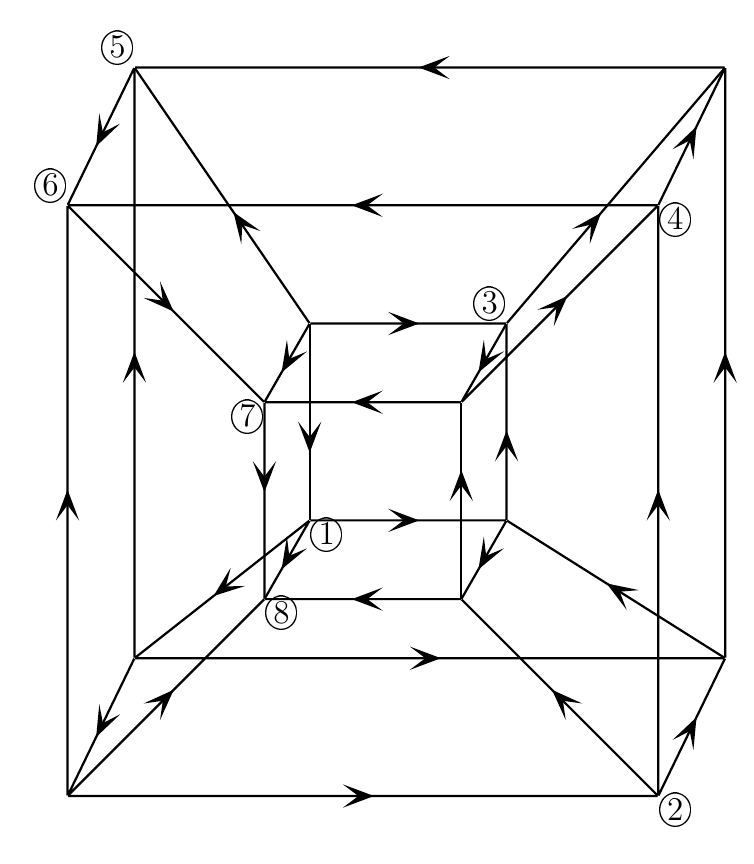
\begin{tikzpicture}[scale=2.5]
    

\pgfarrowsdeclare{mytipnew}{mytipnew} 
{ 
  \arrowsize=0.2pt 
  \advance\arrowsize by .5\pgflinewidth 
  \pgfarrowsleftextend{-4\arrowsize-2\pgflinewidth} 
  \pgfarrowsrightextend{2\pgflinewidth} 
} 
{ 
  \arrowsize=1pt 
  \advance\arrowsize by .5\pgflinewidth 
  \pgfsetdash{}{0pt} % do not dash 
  \pgfsetroundjoin   % fix join 
  \pgfsetroundcap    % fix cap 
  \pgfpathmoveto{\pgfpoint{-4\arrowsize}{3\arrowsize}}
  \pgfpathlineto{\pgfpoint{4\arrowsize}{0\arrowsize}}
  \pgfpathlineto{\pgfpoint{-4\arrowsize}{-3\arrowsize}}
  \pgfpathlineto{\pgfpoint{0\arrowsize}{0\arrowsize}}
  \pgfpathlineto{\pgfpoint{-4\arrowsize}{3\arrowsize}}
%   \pgfusepathqstroke 
  \pgfusepathqfill
}
 \tikzset{
  % style to apply some styles to each segment of a path
  every node/.style={draw,circle,inner sep=0pt,minimum size=0pt},
  on each segment/.style={
     decorate,
     decoration={
      show path construction,
      moveto code={},
      lineto code={
         \path [#1]
         (\tikzinputsegmentfirst) -- (\tikzinputsegmentlast);
      },
      curveto code={
         \path [#1] (\tikzinputsegmentfirst)
         .. controls
         (\tikzinputsegmentsupporta) and (\tikzinputsegmentsupportb)
         ..
         (\tikzinputsegmentlast);
      },
      closepath code={
         \path [#1]
         (\tikzinputsegmentfirst) -- (\tikzinputsegmentlast);
      },
     },
  },
  mid arrow/.style={postaction={decorate,decoration={
         markings,
         mark=at position .5 with {{\arrow[#1]{mytipnew}}},
      }}},
  near arrow/.style={postaction={decorate,decoration={
         markings,
         mark=at position .4 with {{\arrow[#1]{mytipnew}}},
      }}},
  far arrow/.style={postaction={decorate,decoration={
         markings,
         mark=at position .6 with {{\arrow[#1]{mytipnew}}},
      }}},
 }


\tikzstyle{edge} = [draw,thick,postaction={on each segment={mid arrow=black}},black]
\tikzstyle{edgefar} = [draw,thick,postaction={on each segment={far arrow=black}},black]
\tikzstyle{edgenear} = [draw,thick,postaction={on each segment={near arrow=black}},black]
\newcommand{\mycircle}[1]{\large{\raisebox{.5pt}{\textcircled{\raisebox{-.9pt} {#1}}}}}
\path(0,0) node[label=below right:{\mycircle{8}}] (v0) {}
     (0,1) node (v1)[label=below left:\mycircle{7}] {}
     (1,0) node (v2) {}
     (1,1) node (v3) {}
     (0.23, 0.4) node (v4)[label=below right:\mycircle{1}] {}
     (0.23,1.4) node (v5) {}
     (1.23,0.4) node (v6) {}
     (1.23,1.4) node (v7)[label=above left:\mycircle{3}] {}
     (-1,-1) node (v8) {}
     (-1,2) node (v9)[label=above left:\mycircle{6}] {}
     (-0.66,2.7) node (v13)[label=above left:\mycircle{5}] {}
     (-0.66,-0.3) node (v12) {}
     (2,-1) node (v10)[label=below right:\mycircle{2}] {}
     (2.34,-0.3) node (v14) {}
     (2,2) node (v11)[label=below right:\mycircle{4}] {}
     (2.34,2.7) node (v15) {};
% \node[above of=v1,node distance=0.2in] (v1l) {2};
\draw[edge]
%  (v1) -- (v0)
 (v2) -- (v0)
%  (v2) -- (v3)
 (v3) -- (v1)
 (v3) -- (v11)
 (v4) -- (v0)
 (v4) -- (v6)
 (v4) -- (v12)
 (v5) -- (v1)
%  (v5) -- (v4)
 (v5) -- (v7)
%  (v5) -- (v13)
 (v6) -- (v2)
%  (v6) -- (v7)
 (v7) -- (v3)
%  (v7) -- (v15)
 (v8) -- (v0)
 (v8) -- (v9)
 (v8) -- (v10)
 (v9) -- (v1)
 (v10) -- (v2)
 (v10) -- (v11)
 (v10) -- (v14)
 (v11) -- (v9)
 (v11) -- (v15)
 (v12) -- (v8)
 (v12) -- (v13)
 (v12) -- (v14)
 (v13) -- (v9)
 (v14) -- (v6)
 (v14) -- (v15)
 (v15) -- (v13);
 \draw[edgenear] (v5) -- (v13) (v7) -- (v15) (v1) -- (v0) (v6) -- (v7);
 \draw[edgefar] (v2) -- (v3) (v5) -- (v4);
    %  \draw[edge] (v1) -- (v0);
    %  \draw[edge] (v2) -- (v0);
    %  \draw[edge] (v2) -- (v3);
    %  \draw[edge] (v3) -- (v1);
    %  \draw[edge] (v3) -- (v11);
    %  \draw[edge] (v4) -- (v0);
    %  \draw[edge] (v4) -- (v6);
    %  \draw[edge] (v4) -- (v12);
    %  \draw[edge] (v5) -- (v1);
    %  \draw[edge] (v5) -- (v4);
    %  \draw[edge] (v5) -- (v7);
    %  \draw[edge] (v5) -- (v13);
    %  \draw[edge] (v6) -- (v2);
    %  \draw[edge] (v6) -- (v7);
    %  \draw[edge] (v7) -- (v3);
    %  \draw[edge] (v7) -- (v15);
    %  \draw[edge] (v8) -- (v0);
    %  \draw[edge] (v8) -- (v9);
    %  \draw[edge] (v8) -- (v10);
    %  \draw[edge] (v9) -- (v1);
    %  \draw[edge] (v10) -- (v2);
    %  \draw[edge] (v10) -- (v11);
    %  \draw[edge] (v10) -- (v14);
    %  \draw[edge] (v11) -- (v9);
    %  \draw[edge] (v11) -- (v15);
    %  \draw[edge] (v12) -- (v8);
    %  \draw[edge] (v12) -- (v13);
    %  \draw[edge] (v12) -- (v14);
    %  \draw[edge] (v13) -- (v9);
    %  \draw[edge] (v14) -- (v6);
    %  \draw[edge] (v14) -- (v15);
    %  \draw[edge] (v15) -- (v13);
    %  \draw[selected edge] (v4) -- (v10);
    %  \draw[selected edge] (v10) -- (v7);
    %  \draw[selected edge] (v7) -- (v11);
    %  \draw[selected edge] (v11) -- (v13);
    %  \draw[selected edge] (v13) -- (v9);
    %  \draw[selected edge] (v9) -- (v1);
    %  \draw[selected edge] (v1) -- (v0);
 \end{tikzpicture}
 }
 \caption{The only 4-AUSO (up to an isomorphism) on which HPI performs $8$ vertex evaluations. The $8$ vertices are numbered in sequence. This AUSO does not satisfy the Holt-Klee conditions. Notice, for example, that the inner $3$-AUSO does not have $3$ vertex-disjoint paths from source to sink.}
 \label{fig:4auso-8hpi}
\end{figure}


While the improved upper bounds above become the tightest strong worst-case bounds known for the PI family (since HPI is deterministic), our enumerated list of AUSOs also facilitates the analysis of a randomised variant of BSPI in which RPI is used within each batch. We denote this variant BSPI-R. We are not aware of relaxations such as the order regularity problem for analysing BSPI-R; our direct enumeration of AUSOs provides the first non-trivial bounds. We find that the expected number of iterations RPI takes on $3$-AUSOs is at most $4.7778$ and on $4$-AUSOs is at most $6.5544$ (in both cases the Holt-Klee conditions do not lead to tighter bounds). Although these bounds---maximised over all AUSOs in the corresponding family---are smaller than those for HPI, there do exist AUSOs on which HPI dominates RPI. The distributions of the number of iterations taken by RPI and HPI on $3$- and $4$-AUSOs are shown in Figure~\ref{fig:3-4-auso-bounds}. Reusing the recursion shown by Kalyanakrishnan \textit{et al.}~\shortcite{Kalyanakrishnan+MG-bspi:2016}, we obtain $6.5544^{n/4} < 1.6001^{n}$ as a bound on the number of iterations taken by BSPI-R on $2$-action MDPs. This strong upper bound is the tightest shown to date for the PI family for $k = 2$. 
%The generalisation---$k^{0.6782n}$ for $k$-action MDPs---is not as tight as 
For $k \geq 3$, %the $(O(\log k))^{n}$ bound of Gupta and Kalyanakrishnan~\shortcite{Kalyanakrishnan+Gupta} is 
the tightest such bounds are
$(O(\log k))^{n}$~\cite{Kalyanakrishnan+Gupta}.


\begin{figure}[t]
\centering%%% not \center
\mbox{
\subfigure[3-AUSO]{%
\label{fig:auso3}%
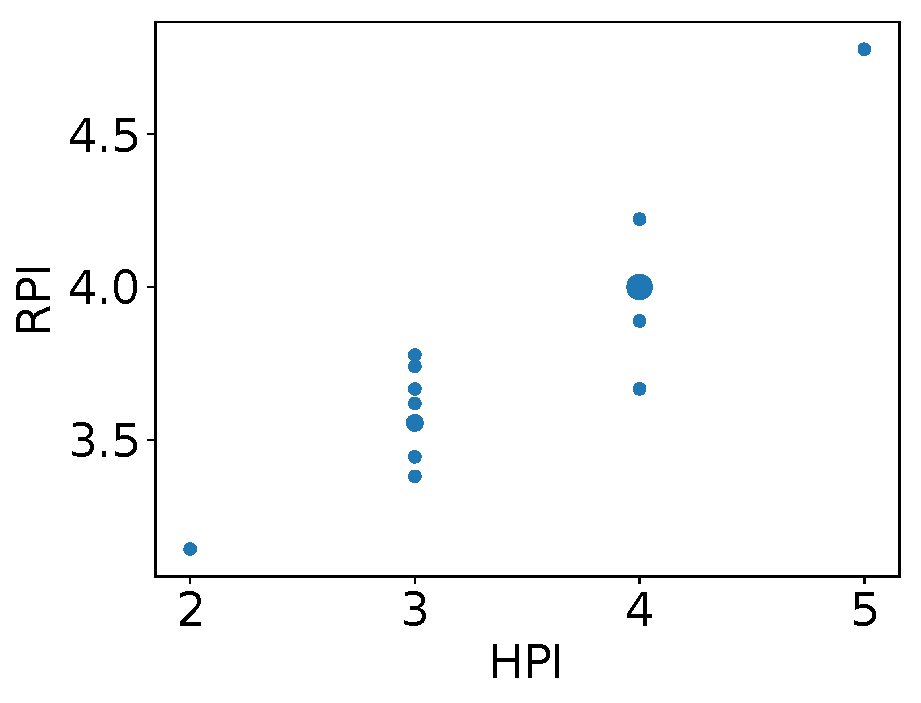
\includegraphics[width=0.24\textwidth]{figs/3-auso-scatter}%
}%
\subfigure[3-AUSO (Holt-Klee)]{%
\label{fig:hkauso3}%
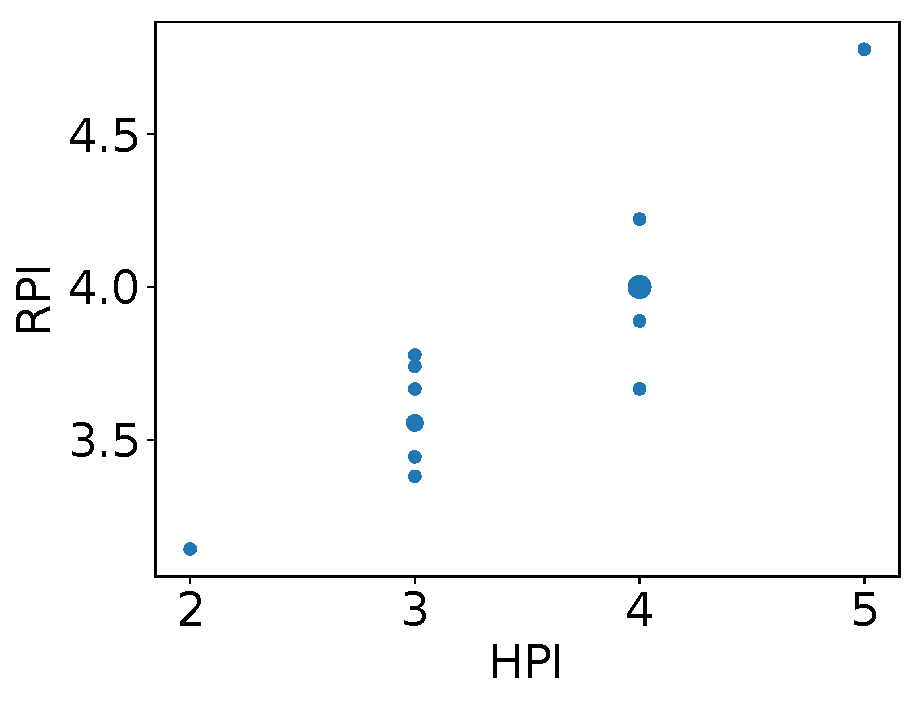
\includegraphics[width=0.24\textwidth]{figs/3-hk-auso-scatter}%
}%
}
\mbox{
\subfigure[4-AUSO]{%
\label{fig:auso4}%
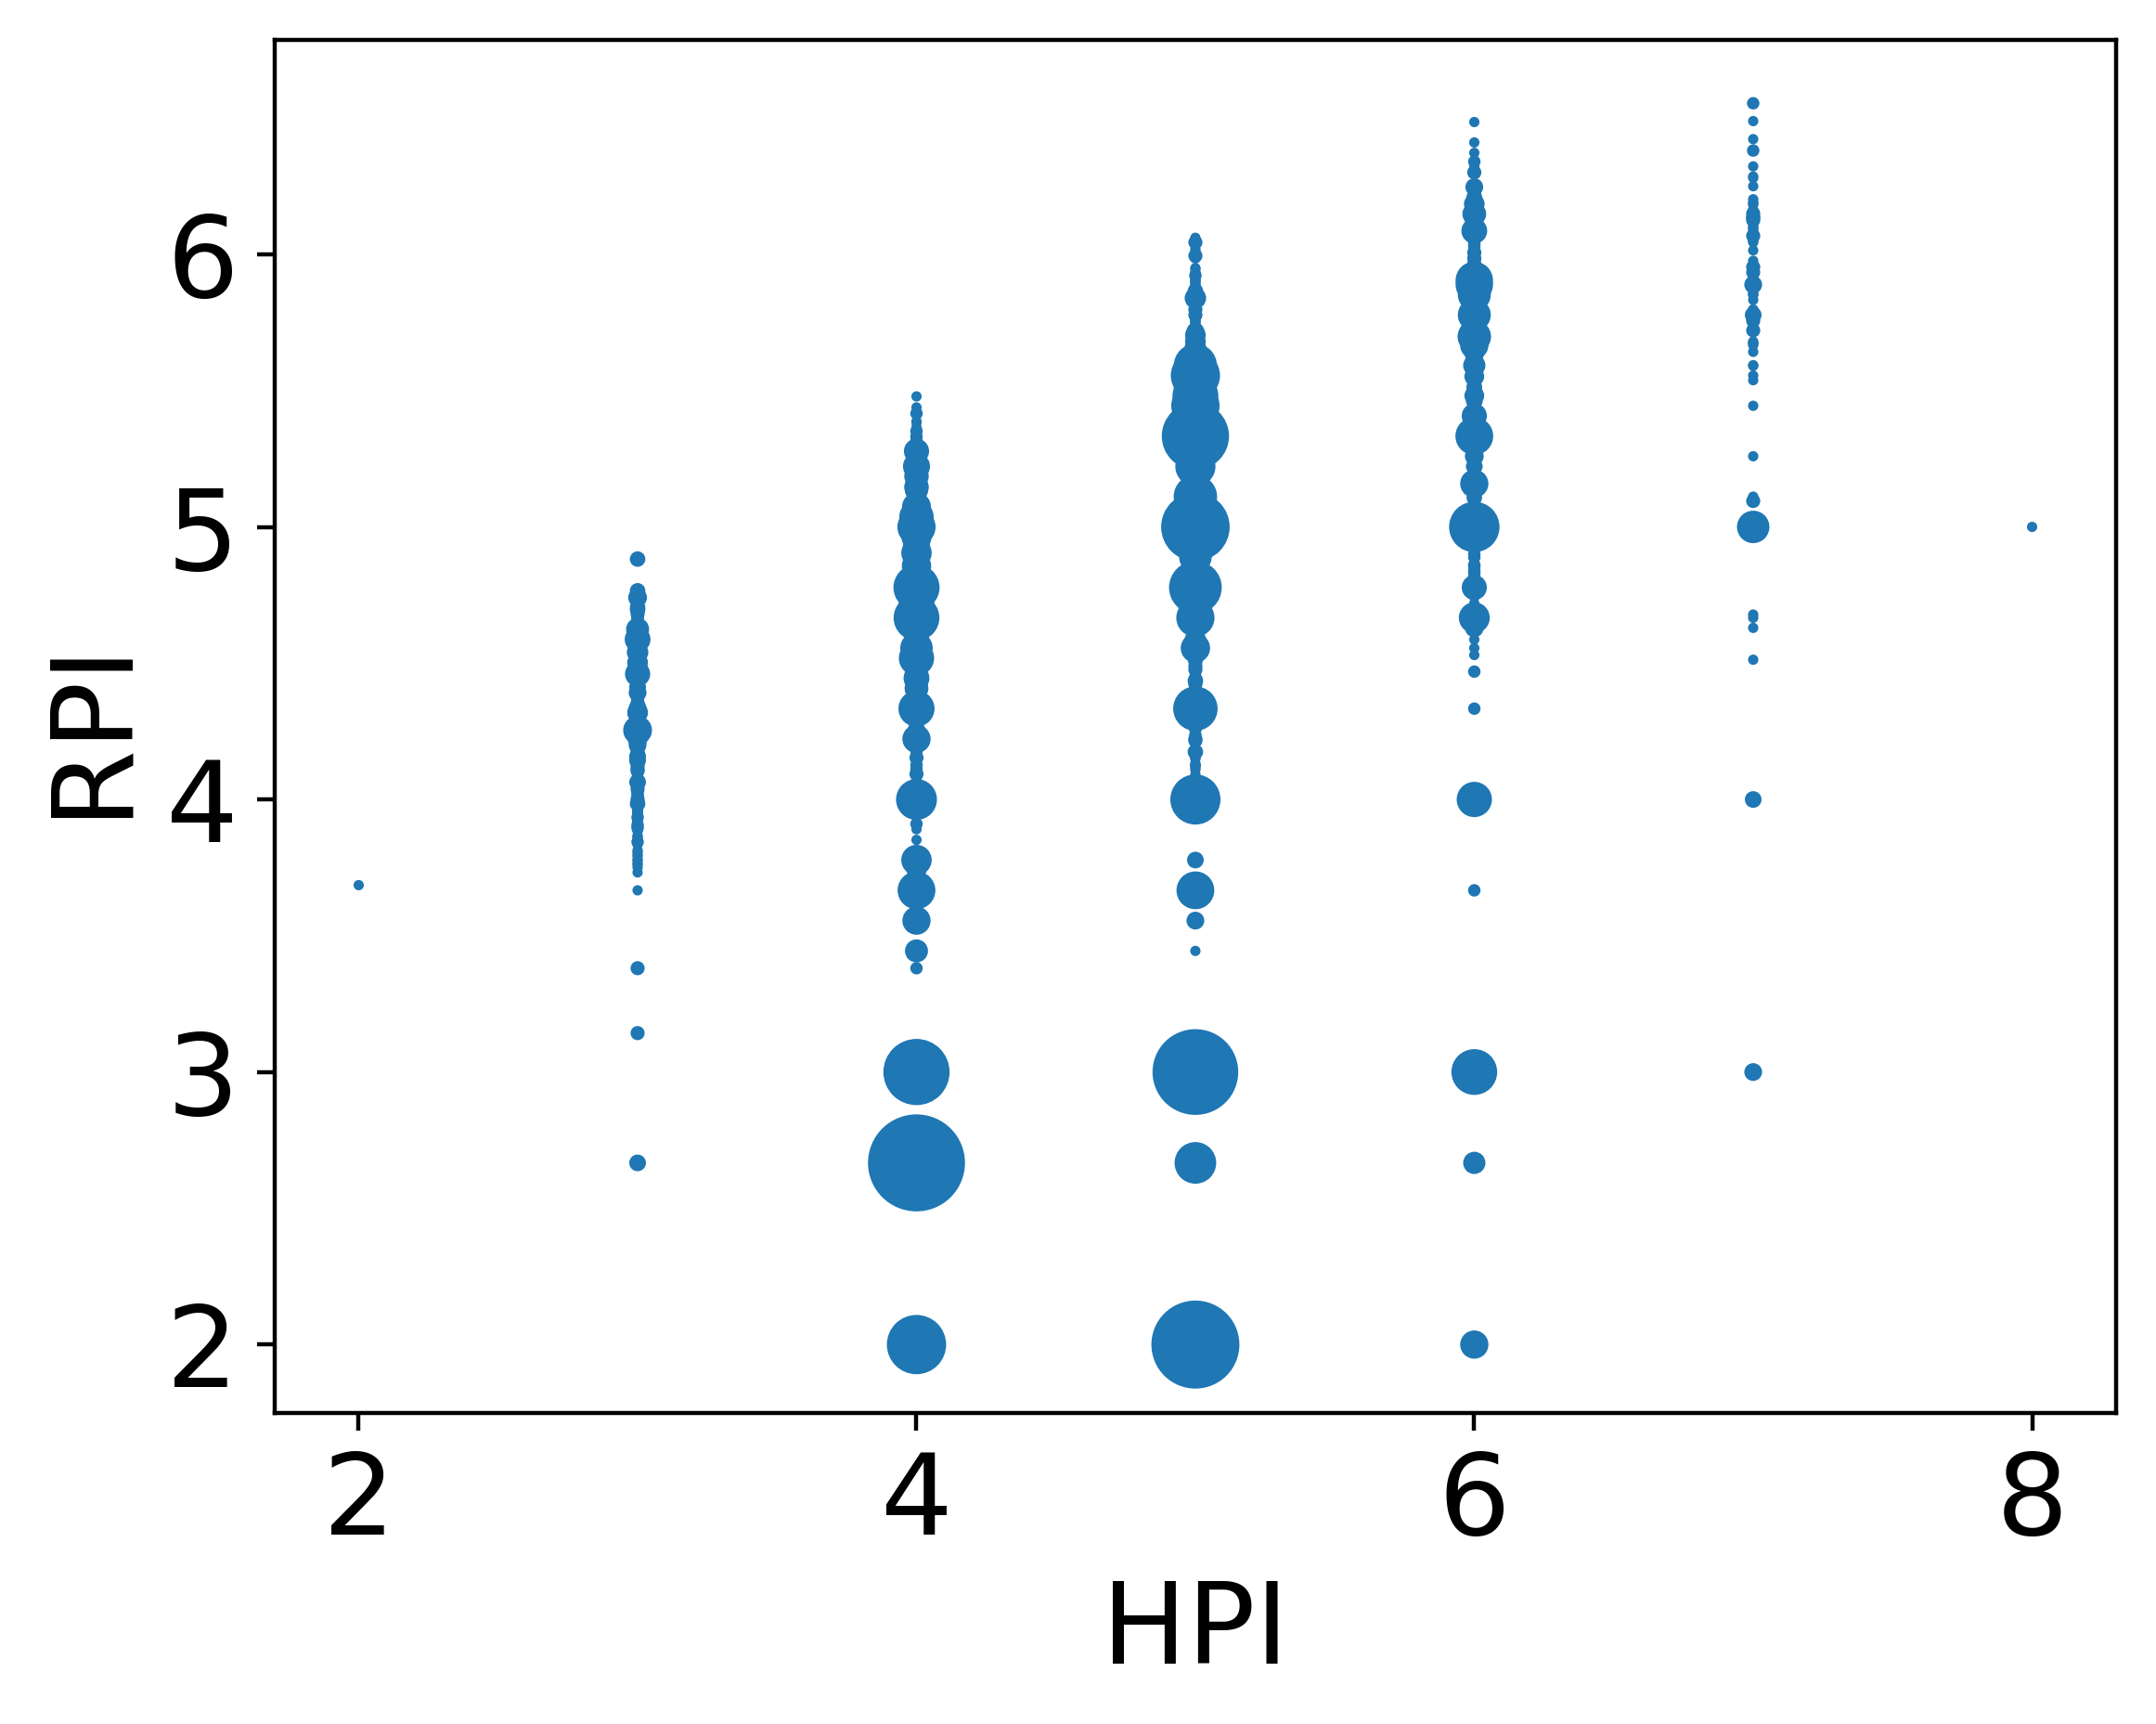
\includegraphics[width=0.24\textwidth]{figs/4-auso-scatter}%
}%
\subfigure[4-AUSO (Holt-Klee)]{%
\label{fig:hkauso4}%
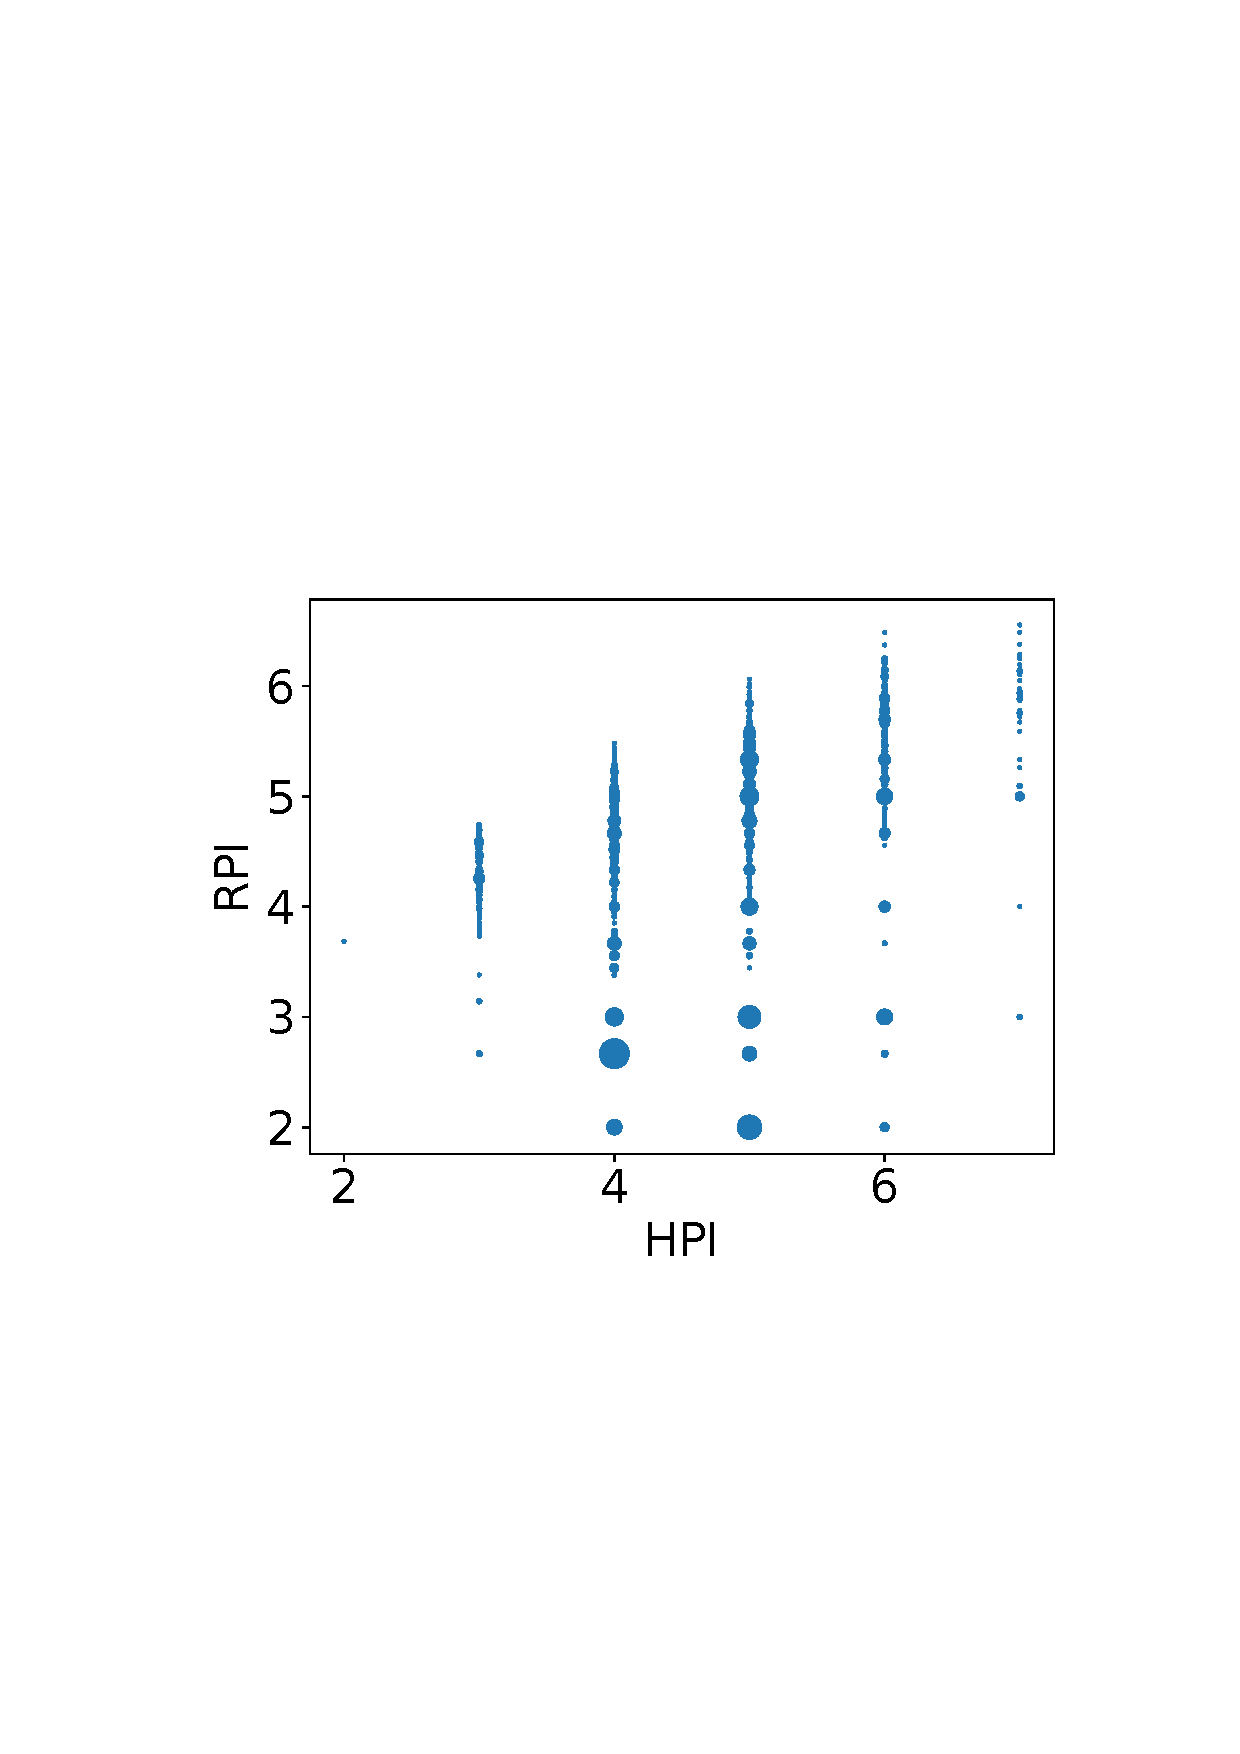
\includegraphics[width=0.24\textwidth]{figs/4-hk-auso-scatter}%
}%
}
\caption{Number of iterations taken by HPI and RPI on instances of different families of AUSOs. The area of each circle is proportional to the number of AUSOs whose HPI- and RPI- iterations are the centre's x and y coordinates, respectively. % For each method the curve is obtained by computing the number of iterations for each instance of the family, and plotting these numbers in non-decreasing order. Thus, for a given point on the x axis, the HPI and RPI iterations plotted might not be for the same instance.
}
\label{fig:3-4-auso-bounds}
\end{figure}



\section{LOWER BOUND}
\label{sec:lowerbound}


  \begin{figure*}[t]
  \centering
  % \scalebox{0.7}
  % {
  % \begin{tikzpicture}[node distance=3cm,auto,scale=0.1,-{Latex[length=3mm,width=2mm]},>=Latex]
  \begin{tikzpicture}[node distance=3cm,auto,scale=0.5,transform shape,
-{Latex[length=1.8mm,width=1mm]},>=Latex]

  % \begin{tikzpicture}[node distance=3cm,auto,scale=0.6, every node/.style={scale=0.6},->]
    % \tikzstyle{state}=[circle,draw=black,minimum size=13mm]
    % \tikzstyle{sink}=[draw=black,minimum size=12mm]
    \tikzset{state/.style={circle,draw=black,minimum size=14mm},
          sink/.style={draw=black,minimum size=12mm}}

    \node[state](n){$n$};
    \node[state,right of=n](n1){$n-1$};
    \node[state,right of=n1](n2){$n-2$};
    \node[right of=n2](e1){\Huge\textbf{...}};
    \node[state,right of=e1](nn2){$2$};
    \node[state,right of=nn2](nn1){$1$};
    \node[state,right of=nn1](nn0'){$0'$};
    \node[sink,right of=nn0'](s1){$\Tilde{1}$};
    
    \node[state,below of=n](n'){$n'$};
    \node[state,right of=n'](n1'){$(n-1)'$};
    \node[state,right of=n1'](n2'){$(n-2)'$};
    \node[right of=n2'](e1'){\Huge\textbf{...}};
    \node[state,right of=e1'](nn2'){$2'$};
    \node[state,right of=nn2'](nn1'){$1'$};
    \node[sink,right of=nn1'](s0){$\Tilde{0}$};
    

    \draw(n) edge [dashed, red] (n1);
    \draw(n1) edge [dashed, red] (n2);
    \draw(nn2) edge [dashed, red] (nn1);
    \draw(nn1) edge [dashed, red] (nn0');
    \draw(nn0') edge node {$-1$} (s1);
    \draw(nn0') to[bend right=20] (n);


    \draw(n') edge (n1');
    \draw(n1') edge (n2');
    \draw(nn2') edge (nn1');
    \draw(nn1') edge (s0);
    
    \draw(n) edge [densely dotted, blue] (n');
    \draw(n1) edge [densely dotted, blue] (n1');
    \draw(nn2) edge [densely dotted, blue] (nn2');
    \draw(nn1) edge [densely dotted, blue] (nn1');
    \draw(n') edge (n2);
    \draw(n1') edge (e1);
    \draw(n2) edge [dashed, red] (e1);
    \draw(n2') edge (e1');
    \draw(nn2') edge (nn0');
    \draw(nn1') edge node {$-1$} (s1);
    \draw(s0) edge [loop right] (s0);
    \draw(s1) edge [loop right] (s1);


  \end{tikzpicture}
  % }
  \caption{Family of MDPs used to prove the lower bound on RPI. Red (dashed) and blue (dotted) edges from states $1, 2,  \dots, n$
  correspond to actions $0$ and $1$, respectively. Black (solid) edges from all others states are equiprobable under both actions.}
  \label{fig:mnc-mdp}
  \end{figure*}

%   \draw(n) edge node {0} (n1);
%   \draw(n1) edge node {0} (n2);
%   \draw(nn2) edge node {0} (nn1);
%   \draw(nn1) edge node {0} (nn0');
%   \draw(n) edge node{1} (n');
%   \draw(n1) edge node{1} (n1');
%   \draw(nn2) edge node{1} (nn2');
%   \draw(nn1) edge node{1} (nn1');
%   \path [->]
%   (s0)[loop, -{Latex[length=3mm,width=2mm]}] edge (s0);


Melekopoglou and Condon~\shortcite{Melekopoglou+Condon:1994} derived the first exponential lower bound for PI by analysing runs of Simple PI on a family of $2$-action MDPs, parameterised by the number of states $n$. We  use the same family of MDPs to show a linear lower bound on the expected number of policies evaluated by RPI~\cite{Mansour+Singh:1999}.

The MDP $M_n = (S, A, P, R, \gamma)$, for $n \geq 2$, is
shown in Figure~\ref{fig:mnc-mdp} and explained below. 
%$\mathcal{M}=\{ M_n | n\ge 2\}$
%defined as $M_n=(S, A, P, R, \gamma)$ with 
In $M_{n}$, there are $3$ types of states in the set $S=\{1, 2, \dots, n\} \cup \{ 0^{\prime}, 1^{\prime}, \dots, n^{\prime}\} \cup \{\Tilde{0}, \Tilde{1}\}$. The action set is $A=\{0, 1\}$. States labelled $i$ have deterministic transitions: depending on the action, the next state 
is either $i-1$ or $i^{\prime}$ for $i\ge 2$. From states labelled $i^{\prime}$, regardless of the action taken, the next state is picked uniformly at random from $(i-1)^{\prime}$ and $(i-2)$ for $i \ge 3$. States $\Tilde{0}$ and $\Tilde{1}$ are sinks; the agent stays in them forever once they are reached. There is a reward of $-1$ on entering $\Tilde{1}$ from $0^{\prime}$ or $1^{\prime}$. All other rewards are zero. The transitions that make up the corner cases are shown in Figure~\ref{fig:mnc-mdp}. As in the original construction~\cite{Melekopoglou+Condon:1994}, we use $\gamma = 1$. However, it can be verified that the switches made by PI---which depend solely on the $Q$ function---remain the same for 
$\gamma < 1$. 

%all $\gamma \in (\frac{2^n}{2^n+1}, 1]$. 

%\textcolor{red}{Explain how to me (separately).}


Strictly speaking, $M_n$ has $2n+3$ states and hence $2^{2n+3}$ policies. However, there are only $n$ states where the action non-trivially affects the outcome of the next transition. The remaining states are "dummy". Formally, for a policy $\pi$ and state $s\in \{ 0^{\prime}, 1^{\prime}, \dots, n^{\prime}\} \cup \{\Tilde{0}, \Tilde{1}\}$ such that $\pi(s)=0$, we get $Q^{\pi}(s,0)=Q^{\pi}(s,1)=V^{\pi}(s)$, and so $T^{\pi}(s) = \emptyset$. Hence $s$ will not be switched. We adopt the convention that we start PI at a policy $\pi^0$ such that all ``dummy'' states $s$ have $\pi^0(s)=0$. The action at these states will remain $0$ in every policy thereafter visited by PI. In our analysis, we only deal with states in $\{1, 2, \dots, n\}$, and we treat policies as mappings from $\{1, 2, \dots, n\}$ to $\{0, 1\}$. Consequently we may represent a policy $\pi$ as a bit-string $w_1w_2{\dots}w_n \in \{0,1\}^n$ where $\pi(s)=w_s$. In this notation, it can be seen that $\pi^0 = 0^n$ and $\pi^{\star} = 10^{n-1}$. We show the following lower bound.
\begin{theorem}
\label{thm:lowerbound}
	Starting from $\pi^0=0^n$, the expected number of policies RPI evaluates on $M_n$ before terminating is at least $\frac{n+1}{2}$.
\end{theorem}
The proof is based on structural properties of $M_{n}$ identified by Melekopoglou and Condon~\shortcite{Melekopoglou+Condon:1994}. We provide the proof in Appendix B in the supplementary material.
%we can only reach policies $\pi$ with $\pi(s)=0$ for all "dummy" states. There are only $2^n$ such policies, characterized by their actions on the states other than the "dummy" states. Henceforth, we assume $\pi: [n] \xrightarrow{} \{0, 1\}$ for any policy $\pi$, with $\pi(s)=0$ implicit for all "dummy" states $s\in S$. \footnote{$[n]$ is shorthand for $\{1, 2, ..., n\}$.}
%Formally, if we define an equivalence relation $\sim$ on the policy space $\Pi$ such that $\pi \sim \pi'$ if and only if $V^\pi=V^{\pi'}$, this relation has only $2^n$ equivalence classes, one for each element in $\Pi' = \{ \pi:\{1, 2, ..., n\}\xrightarrow{} \{0,1\} \}$. Moreover
% 1. WHAT IS THE CONVENTION ABOUT POLICIES, SINCE MANY STATES ARE DUMMY? SHOULD WE ASSUME POLICIES MAP $\{1, 2, \dots, n\}$ TO $\{0, 1\}$?

%We provide a sketch of our proof and the intermediate results. Full proofs, which mainly rely on  structural arguments about $M_{n}$, are provided in Appendix B in the supplemental material.



% \begin{lemma}
% \label{l1}
% For a policy $\pi$ for $M_n$, a state $s$ is switchable if and only if $\sum_{s'\le s}\pi(s) \equiv 0 \mod 2.$
% \end{lemma}


% \begin{definition}
% \label{d2}
%     For a policy $\pi$ for $M_n$, $$f(\pi) \mathrel{\overset{\makebox[0pt]{\mbox{\normalfont\tiny\sffamily def}}}{=}} \min \left(\textsf{states}(T^\pi) \cup \{n+1\}\right).$$
% \end{definition}
% In other words, $f(\pi)$ is defined to be the smallest switchable state if $\pi$ is not optimal, and $n + 1$ if it is $\pi^{\star}$. The lemma below establishes the monotonicity of $f$.

% \begin{lemma}
% \label{l3}
%     If a PI algorithm visits the policies $\pi^0, \pi^1, \dots, \pi^m$ in sequence, then for $1\le i \le m$, $f(\pi^{i-1})\le f(\pi^i)$.
% \end{lemma}


% \begin{lemma}
% \label{l4}
%     If RPI visits the policies $\pi^0, \pi^1, \dots, \pi^m$ in sequence, then for $1\le i \le m$, $t \ge 0$, $$\mathbb{P}\{f(\pi^{i}) - f(\pi^{i-1}) \ge t\} \le \frac{1}{2^t}.$$
% \end{lemma}


% \begin{definition}
%     We define $L(\pi)$ to be the expected number of policies evaluated by RPI when initialised at $\pi$.
% \end{definition}
% Note that even if we start from $\pi^0=\pi^{\star}$, we need to evaluate $\pi^0$ to know that it is optimal. Hence $L(\pi^{\star})=1$. Let $[x]$ denote the set $\{1, 2, \dots, x\}.$
% \begin{definition}
% For $s \in [n + 1]$, we define $N(s) = \min\{L(\pi)|f(\pi)\le s\}$.
% \end{definition} 

% \begin{theorem}
% 	For $s\in [n+1]$, $N(s) \ge n+2-s$.
%     % $N(n+1) = 0$. $N(i) \ge n+2-i$ for $1 \le i \le n$.
% \end{theorem}


\section{EXPERIMENTS}
\label{sec:experiments}



\begin{figure*}[t]
\centering%%% not \center
% \subfigure[Variation with $k$ for $n=10$, $b=5$, made monotonic]{%
% \label{fig:exp-b}%
% 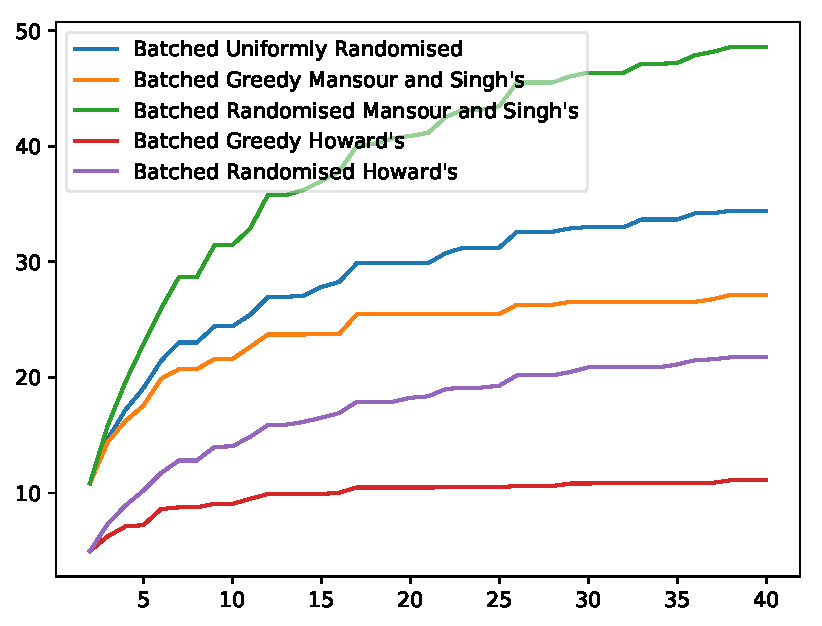
\includegraphics[width=0.5\textwidth]{figs/variation-with-k-monotonized}%
% }
\subfigure[]{%
\label{fig:exp-k}%
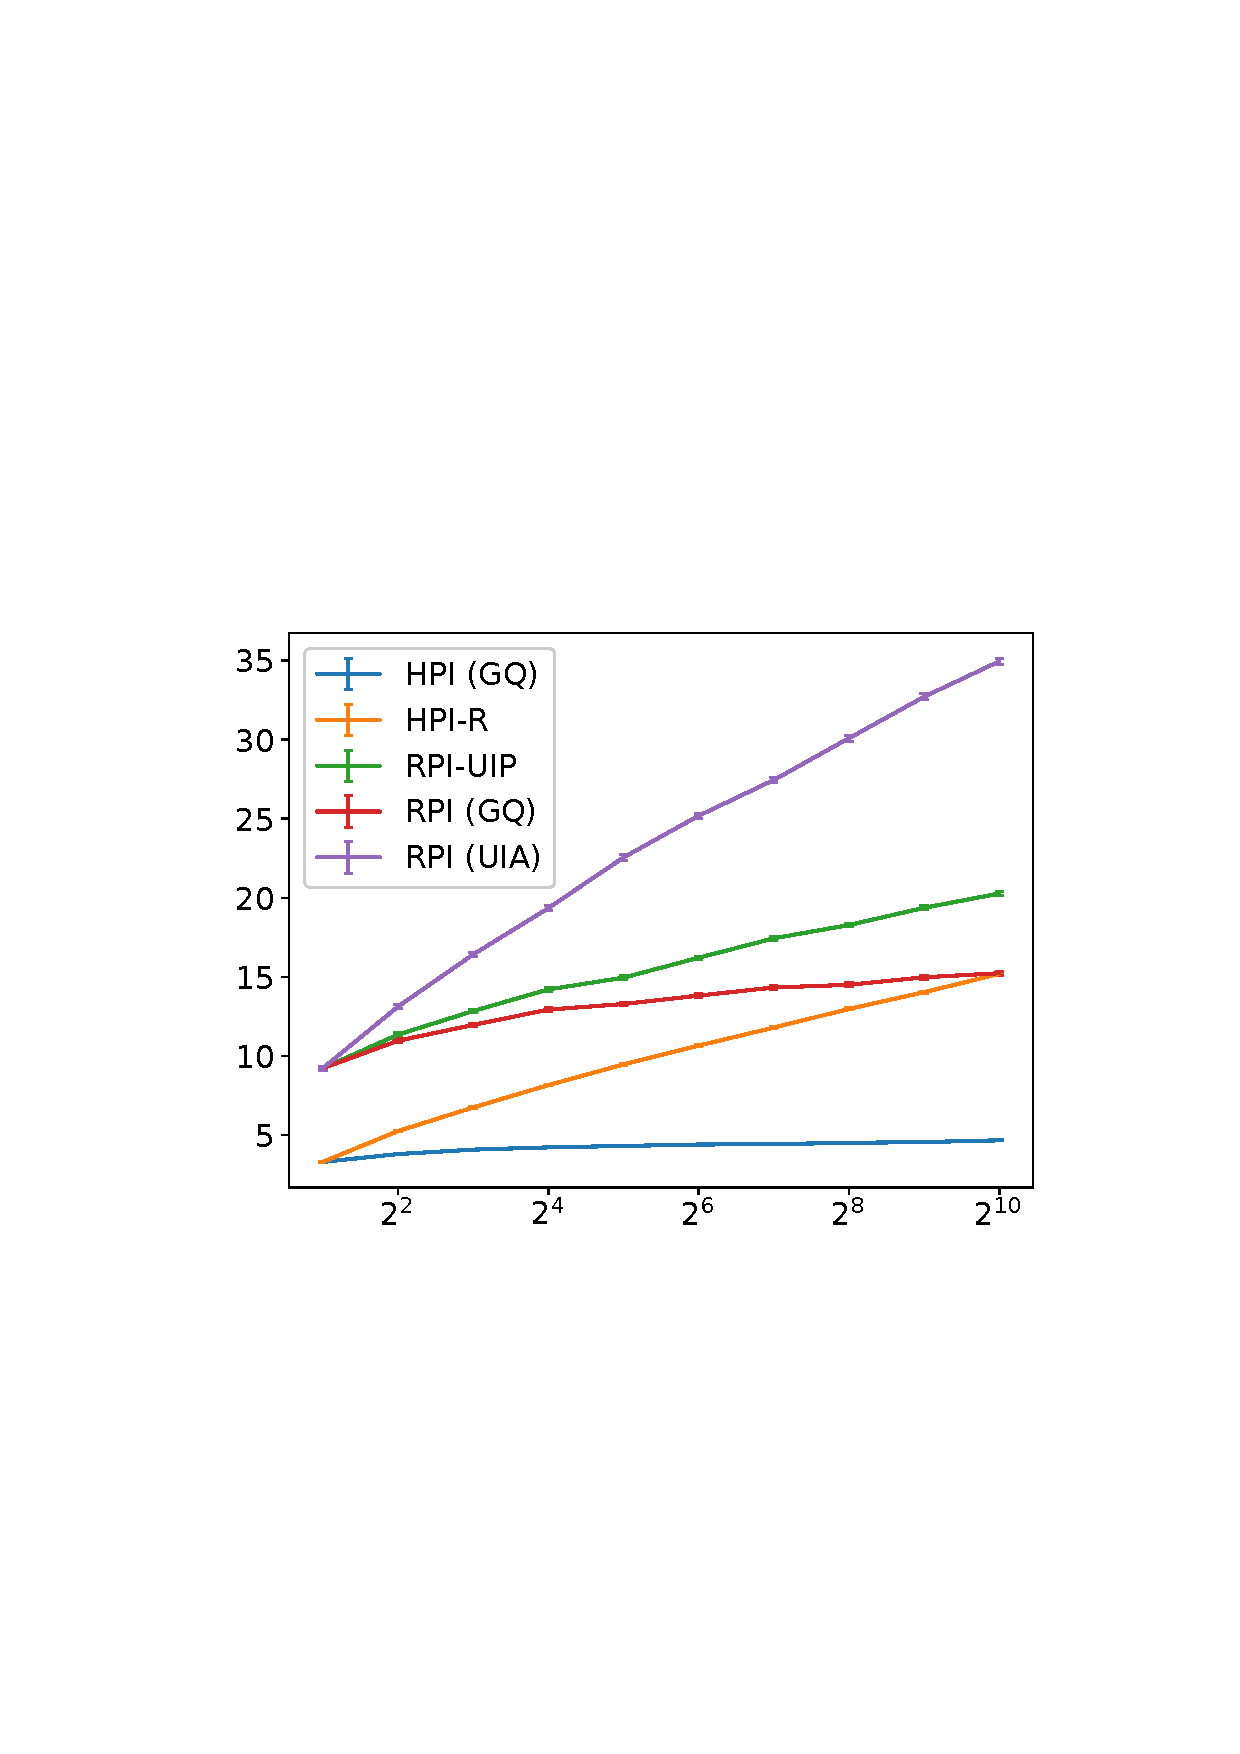
\includegraphics[width=0.25\textwidth]{figs/variation-with-k-logscale}%
}%
\hspace{0.5cm}
\subfigure[]{%
\label{fig:exp-b}%
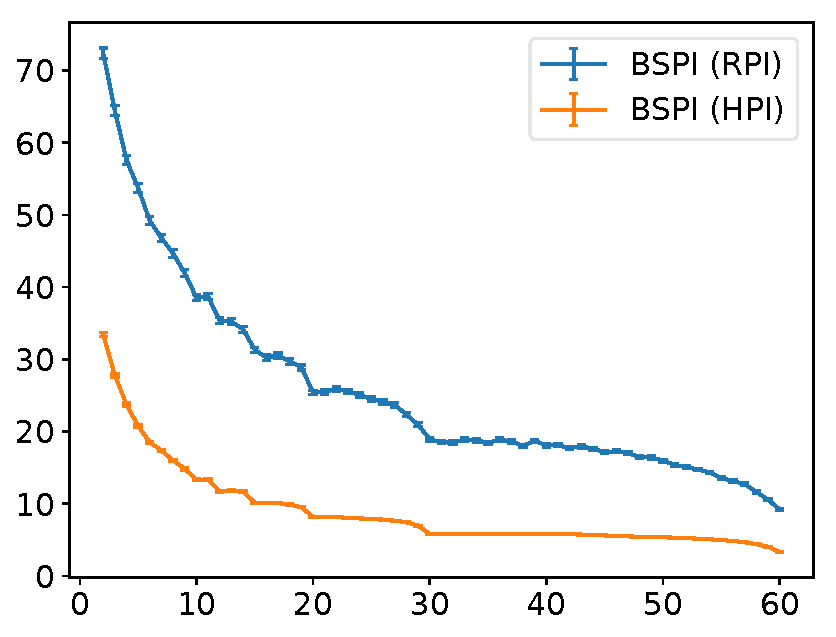
\includegraphics[width=0.25\textwidth]{figs/variation-with-b}%
}%
% \subfigure[Variation with $n$ for $k=6$, $b=5$]{%
% \label{fig:exp-d}%
% 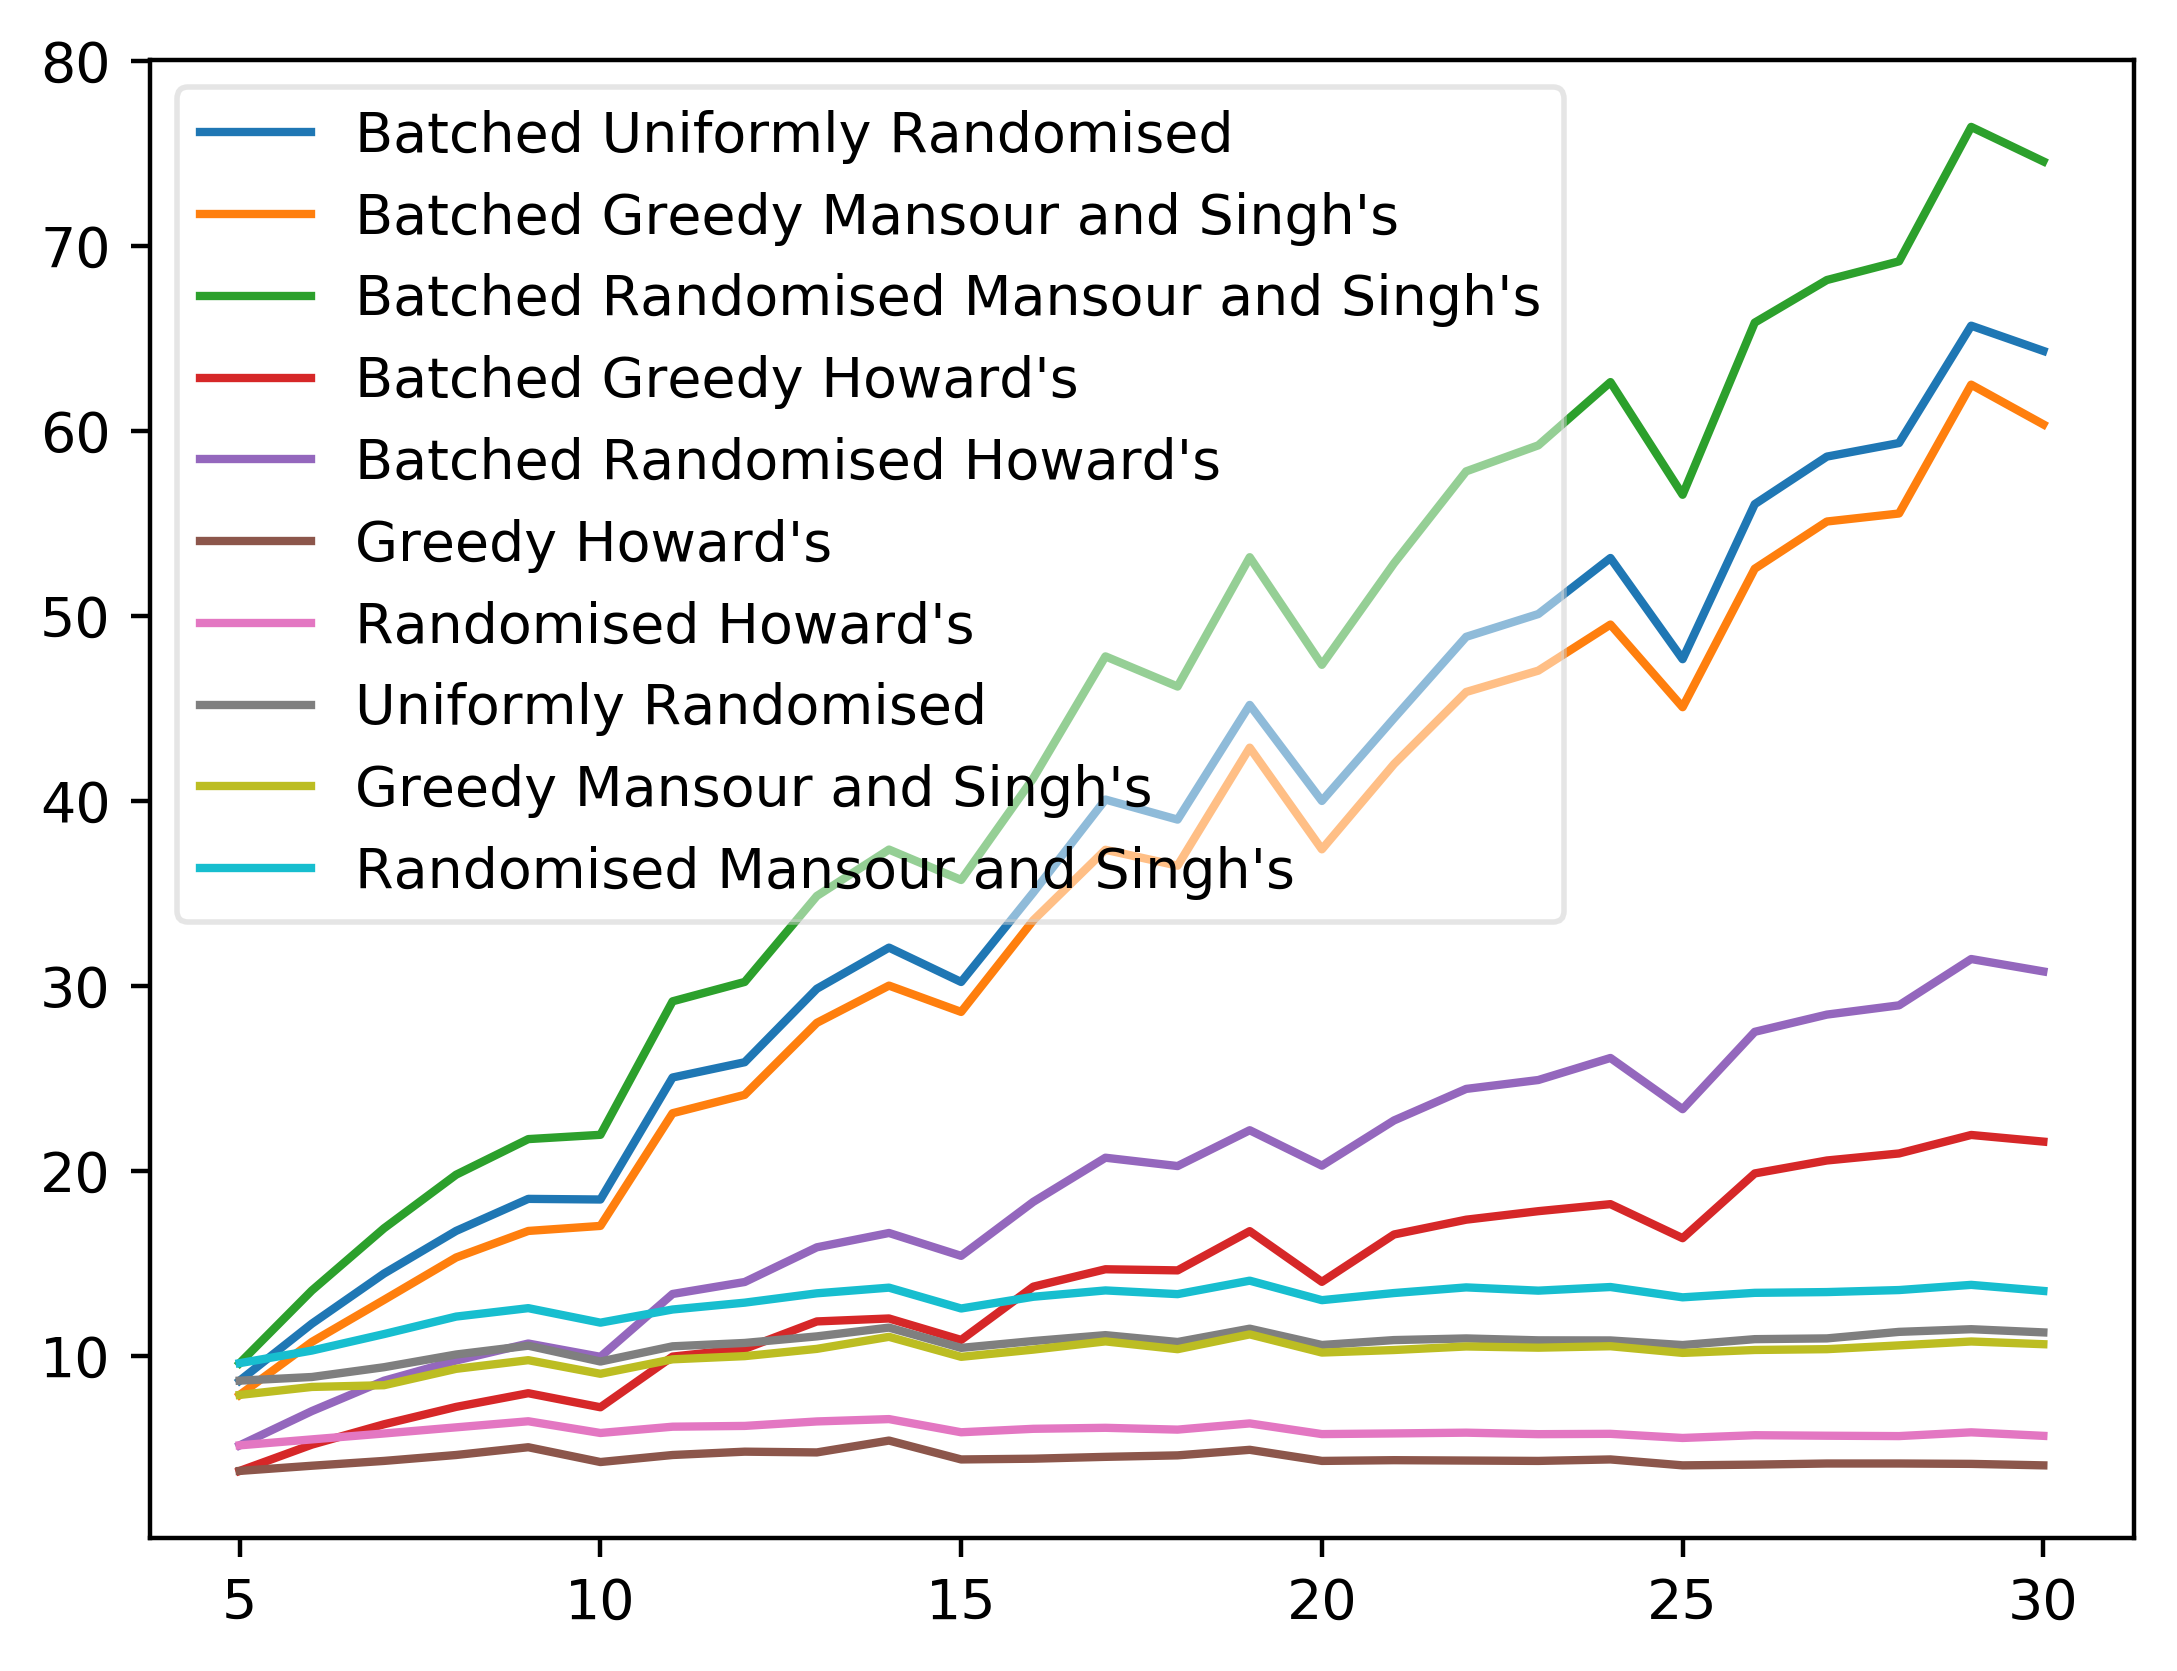
\includegraphics[width=0.5\textwidth]{figs/variation-with-n}%
% }%
\caption{Expected iterations (y axis) against number of actions $k$ in (a) and against batch size $b$ in (b). Each point is an average from 500 independent runs; error bars show one standard error. PI variants HPI (GQ) and RPI (UIA) are described in Section~\ref{sec:experiments}.}
\label{fig:experiments}
\end{figure*}
Interestingly, although the paper by Mansour and Singh~\shortcite{Mansour+Singh:1999} is nearly twenty years old, we are not aware of an experimental comparison between RPI and HPI  published in the literature. We present an experimental comparison of these methods and the variants discussed in this paper, summarising our results in Figure~\ref{fig:experiments}. 

Unlike our theoretical bounds, which are \textit{maximised} over MDPs, each graph plots an \textit{average} over $500$ randomly generated MDPs. In the same manner as  Kalyanakrishnan \textit{et al.}~\shortcite{Kalyanakrishnan+MG-bspi:2016}, we generate an $n$-state, $k$-action MDP by uniformly sampling $n / 5$ possible successors for each of the $nk$ state-action pairs. For each $(s,a,s^{\prime})$ triple thus obtained, the reward $R(s,a,s^{\prime})$ is drawn from a standard normal distribution; $P(s,a,s^{\prime})$ is drawn uniformly from $[0,1]$ and thereafter normalised. The remaining rewards and probabilities are set to $0$. We take $n = 60$ and $\gamma =  0.99$. The starting policy for PI on each MDP is picked uniformly at random.


Figure~\ref{fig:exp-k} compares variants of HPI and RPI as $k$ is varied. Our first observation is that running HPI with greedy action selection based on the $Q$-function (GQ) is by far the most efficient variant.  HPI-R comes second for small values of $k$. Among RPI variants, too, GQ switching performs the best. Note that GQ-switching is only applicable to MDPs, whereas the other variants apply more generally to AUSOs. RPI-UIP consistently takes fewer iterations than than RPI (UIA), a variant of RPI~\cite{Mansour+Singh:1999} in which improving actions are picked uniformly at random from chosen improvable states, which are themselves first selected uniformly at random.

Figure~\ref{fig:exp-b} assesses the effect of using RPI within the batches of BSPI, comparing it with the canonical approach of using HPI~\cite{Kalyanakrishnan+MG-bspi:2016}. This experiment uses $k = 2$. For every fixed batch size $b$, we find that the HPI-based variant performs better in aggregate. Both variants show the same trend: a fairly consistent drop in the number of iterations as $b$ is increased. If it can be proven that a larger batch size implies a tighter upper bound for RPI-based BSPI, it would follow that our bound of $1.6001^{n}$, obtained by analysing $4$-AUSOs, also applies to RPI itself (as it is equivalent to BSPI with a batch size of $n$). Such a result would improve the current bound of $O(1.7172^{n})$ iterations for RPI substantially.

\begin{comment}

~\cite{Mansour+Singh:1999}

\end{comment}

% \begin{figure*}[t!]
% \centering   %%% not \center
% \subfigure[]{
% 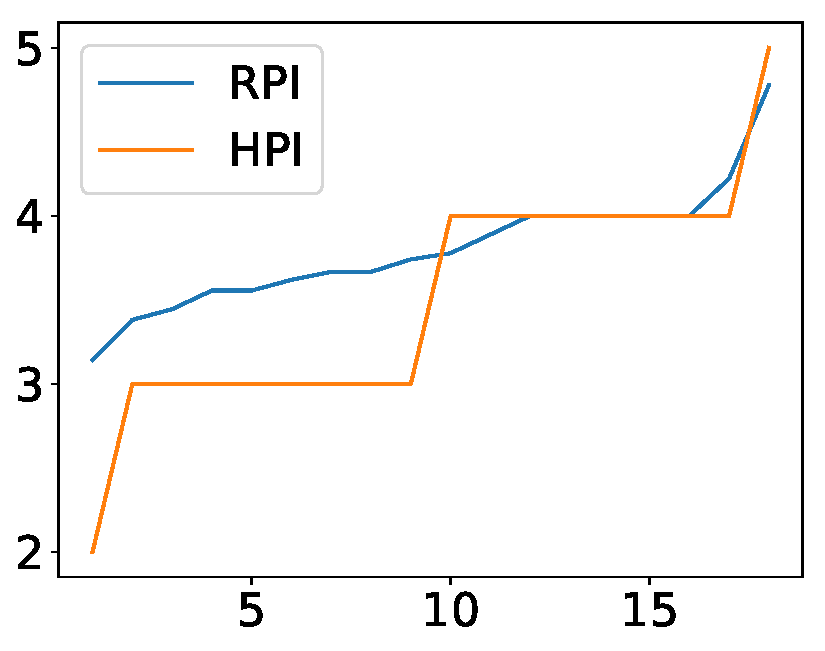
\includegraphics[width=0.245\textwidth]{figs/3-auso}
% }
% \subfigure[]{
% 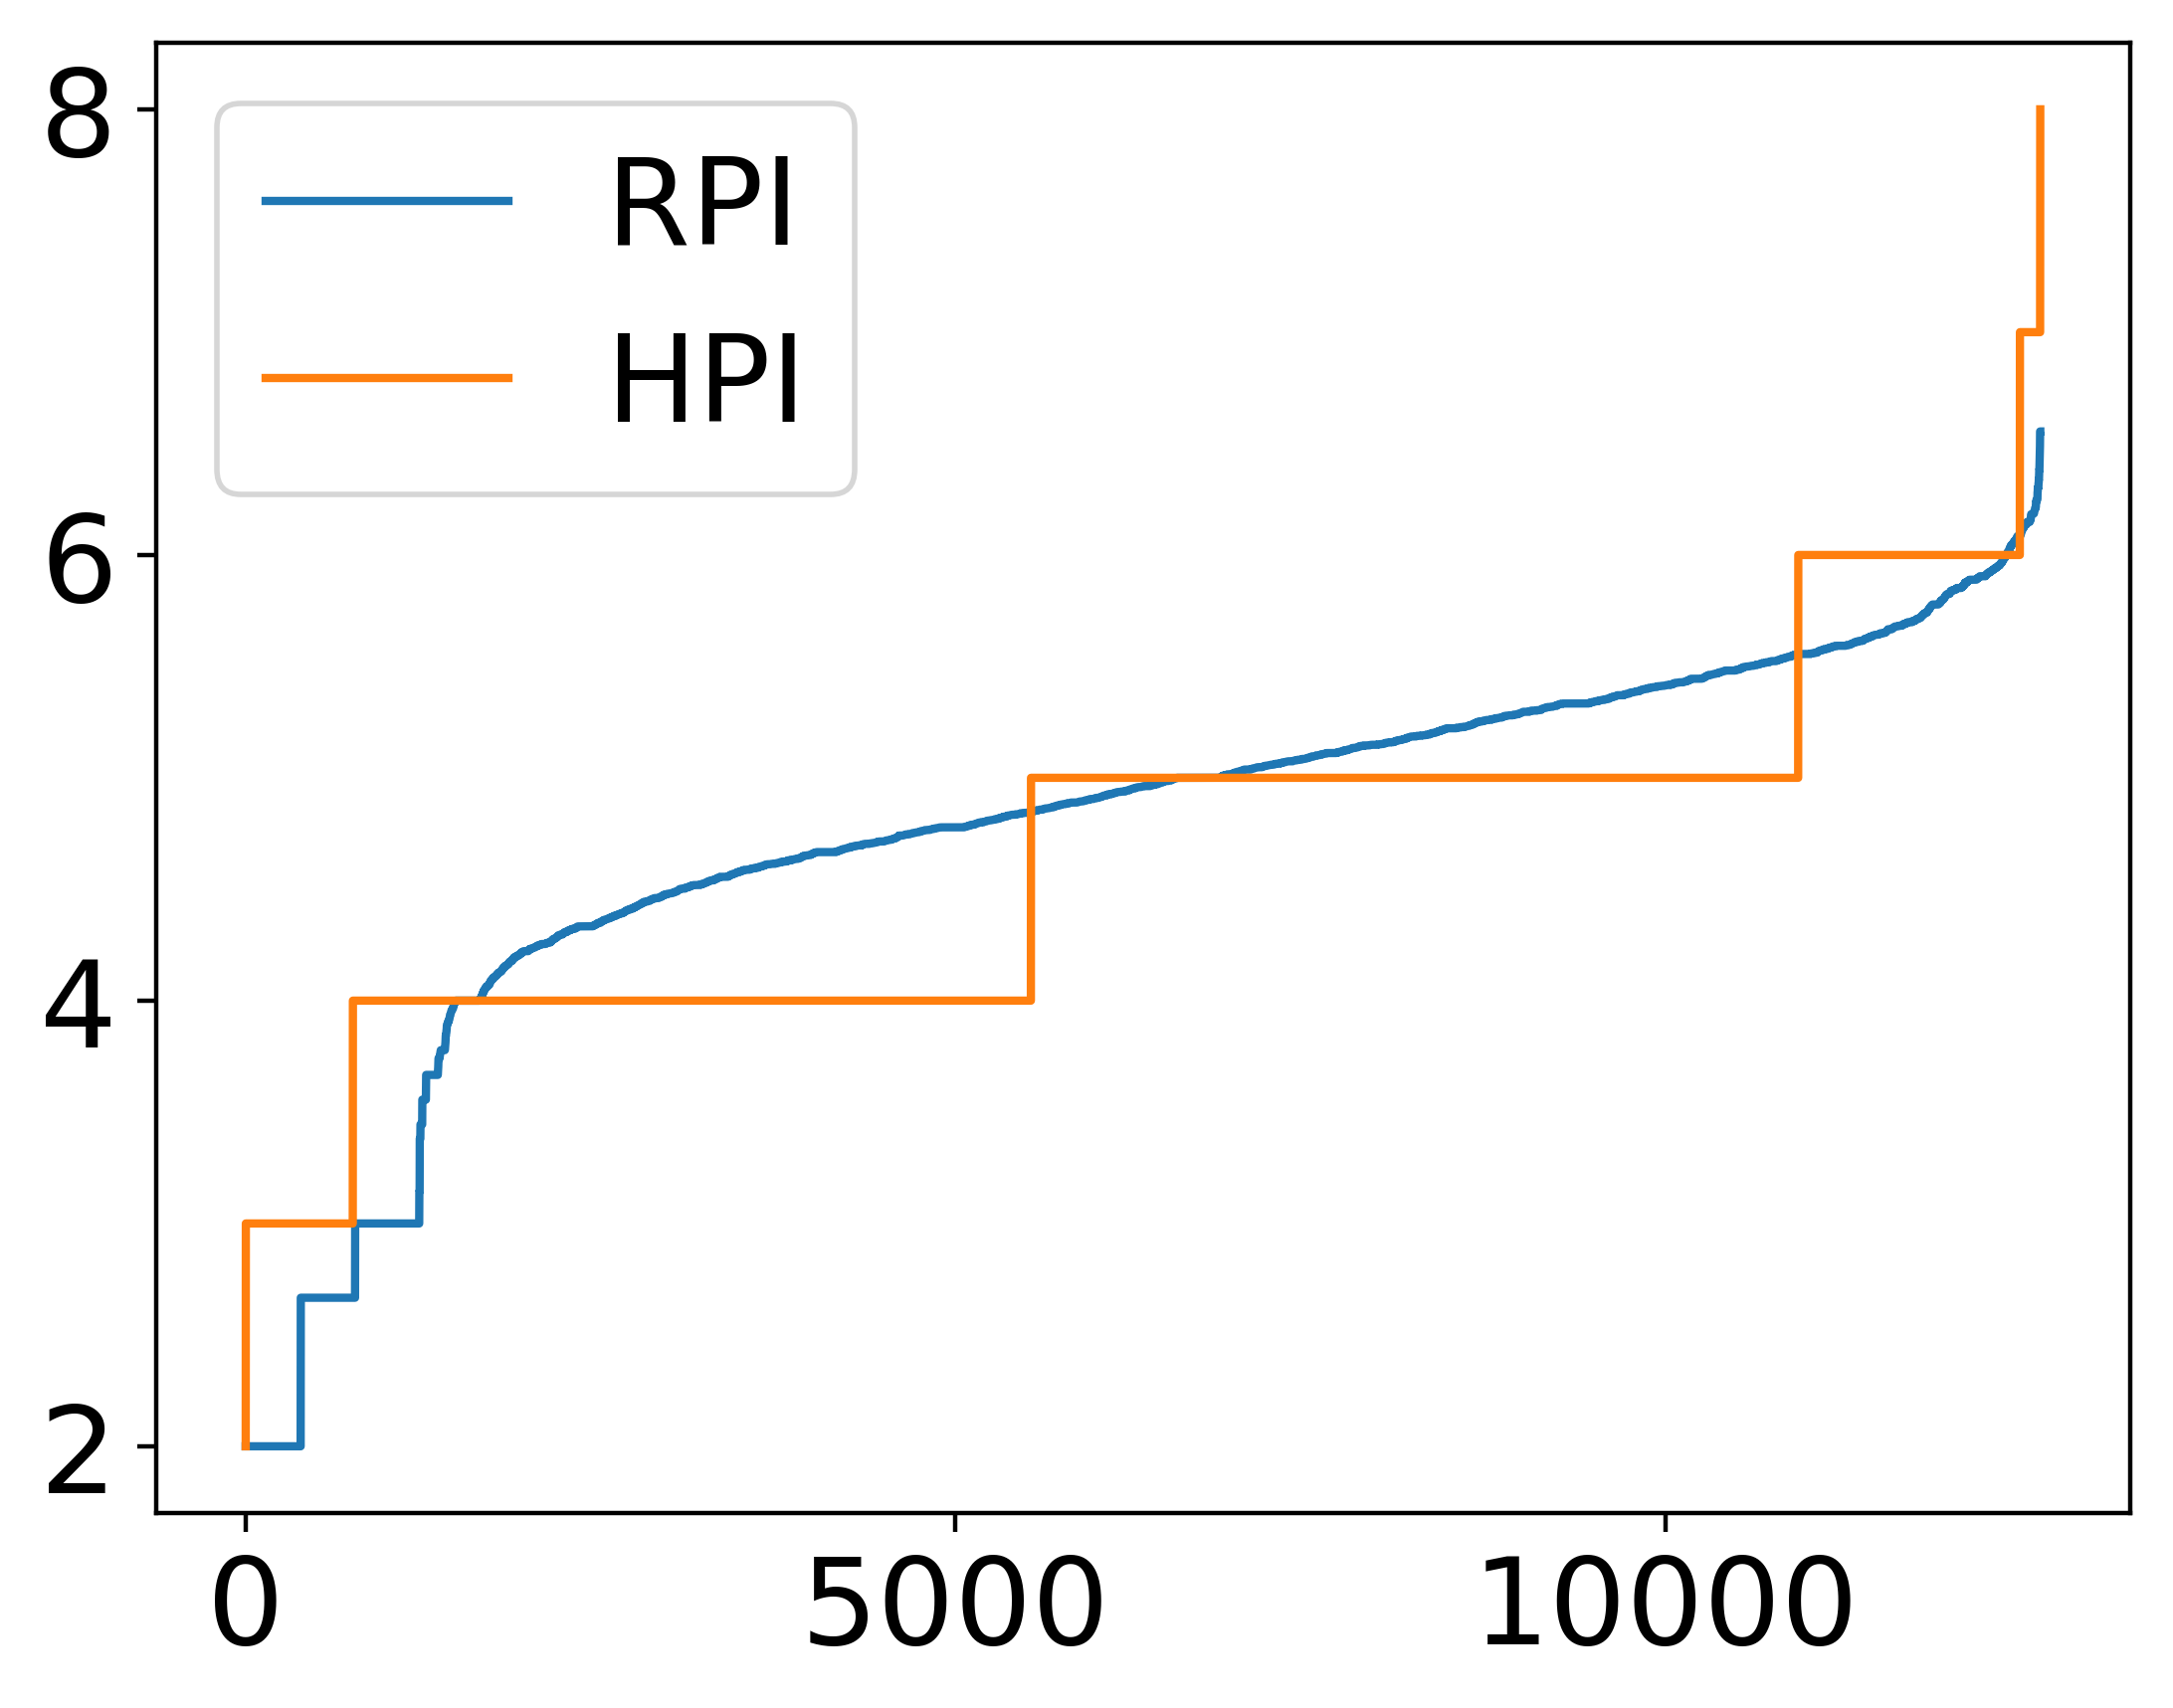
\includegraphics[width=0.245\textwidth]{figs/4-auso}
% }
% \subfigure[]{
% 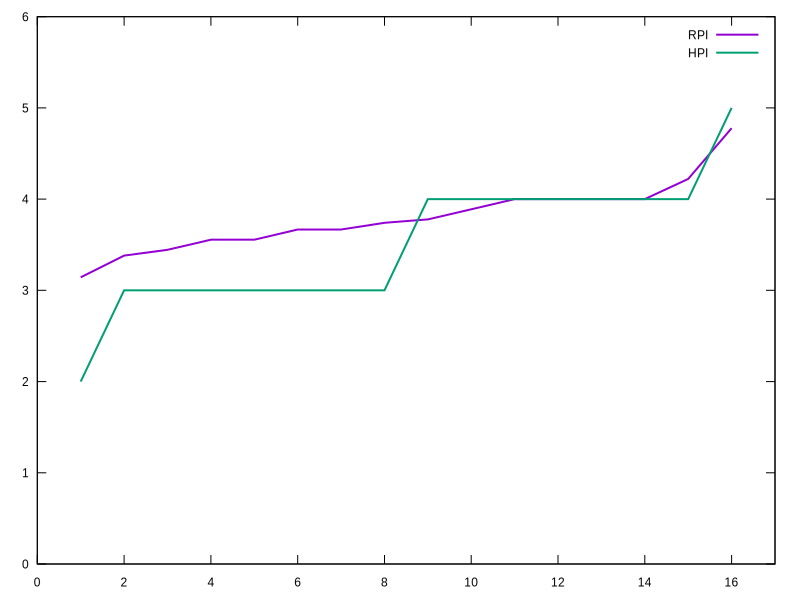
\includegraphics[width=0.245\textwidth]{figs/3-hk-auso}
% }
% \subfigure[]{
% 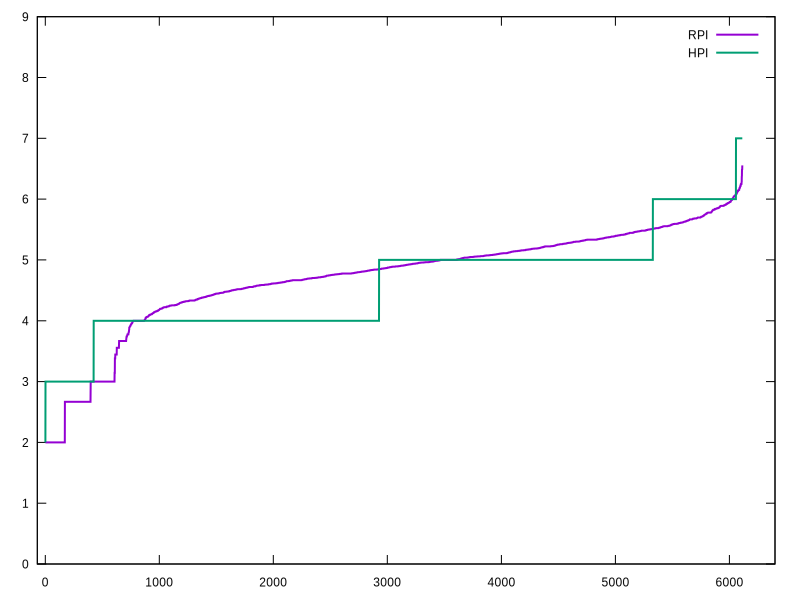
\includegraphics[width=0.245\textwidth]{figs/4-hk-auso}
% }
% \caption{Shivaram will fill out.}
% \label{fig:auso-data}
% \end{figure*}
% 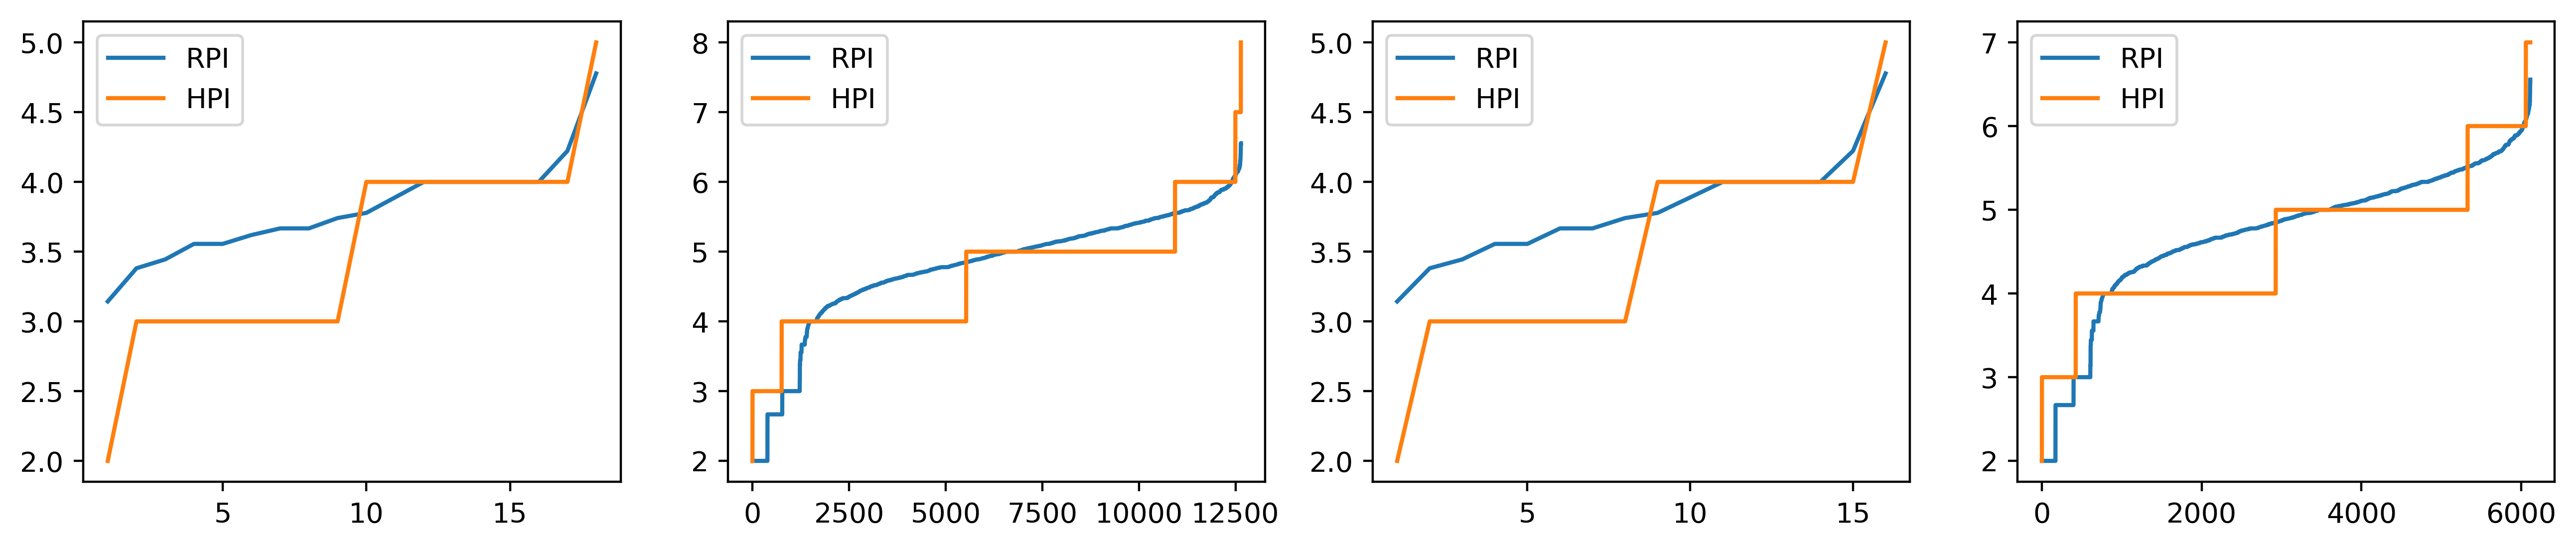
\includegraphics[width=\textwidth]{figs/auso_data.png}



\vspace{-10pt}
\section{DISCUSSION}
\label{sec:conclusion}
Our experimental results are perfectly consistent with our theoretical upper bounds: for $60$-state MDPs, the upper bounds far exceed the ranges plotted in Figure~\ref{fig:experiments}. Yet, curiously, many \textit{trends} seen in practice---even if only on one family of randomly-generated MDPs---are quite opposite to the \textit{trends} among the theoretical bounds. By way of RPI-UIP, we have shown the tightest upper bounds yet for the PI family, which improve upon those for RPI and HPI. Yet, HPI seems to work much better in practice. We may attribute this disparity both to the looseness of the upper bounds, and to our choice of test MDPs. The lower bound we show for RPI matches the tightest for HPI on $2$-action MDPs---but both bounds are only linear. It remains to be seen if there are MDPs on which RPI and HPI have substantially higher complexity.


The analysis provided in this paper does not exploit any properties specific to MDPs, but applies more generally to AUSOs. It would be interesting to analyse RPI specifically on MDPs. For example, it is known that the Simplex method runs in strongly polynomial time on the Linear Program arising from \textit{deterministic} MDPs~\cite{Post+Ye:2013}. To the best of our knowledge,  HPI and RPI have not been shown to enjoy the same guarantee.
\vspace{-10pt}
\subsection*{ACKNOWLEDGEMENTS}
SK was partially supported by   grants from SERB (ECR/2017/002479) and Ubisoft India.
  
%The tightest strong upper bounds currently known for MDP planning are summarised in Table~\ref{tab:summaryofbounds}. The tightest bound for $k = 2$ is of the form $\text{poly}(n) \cdot 1.6059^{n}$. This bound is shown for the Fibonacci Seesaw algorithm, proposed by Szab{\'{o}} and Welzl~\shortcite{Szabo+Welzl:2001} for solving Unique Sink Orientations (USOs). It is known that the policies for 2-action MDPs can be interpreted as vertices of an Acyclic USO (AUSO), whose sink corresponds to an optimal policy. For $k\ge 3$, Kalyanakrishnan and Gupta~\shortcite{Kalyanakrishnan+Gupta} introduced Recursive AUSOs (RAUSOs), which represent the policies of k-action MDPs and extended the Fibonacci Seesaw algorithm to these objects to give a bound of $k^{0.6834n}$. 

% If we look beyond PI, we find even \textit{subexponential} bounds on the expected running time of MDP planning. Bounds of the form $\text{poly}(n, k) \cdot \exp(O(\sqrt{n \log(n)}))$~\cite{Matousek+SW:1996} follow directly from posing MDP planning as a linear program with $n$ variables and $nk$ constraints~\cite{Littman+DK:1995}. The special structure that results when $k = 2$ admits an even tighter bound of $\text{poly}(n) \cdot \exp(2 \sqrt{n})$~\cite{Gartner:2002}.







\bibliographystyle{named}
\bibliography{rpi_bound_uai19}
% \vfill\null
\clearpage

% \appendix

%\setcounter{section}{4}
% \clearpage
\begin{appendices}

\section{AUSO instance from Section 4.1}
\label{app:upperbounds}
% Moved to appendix


 \begin{figure}[H]
 \centering
\scalebox{0.7}
% \scalebox{0.5}
 {
 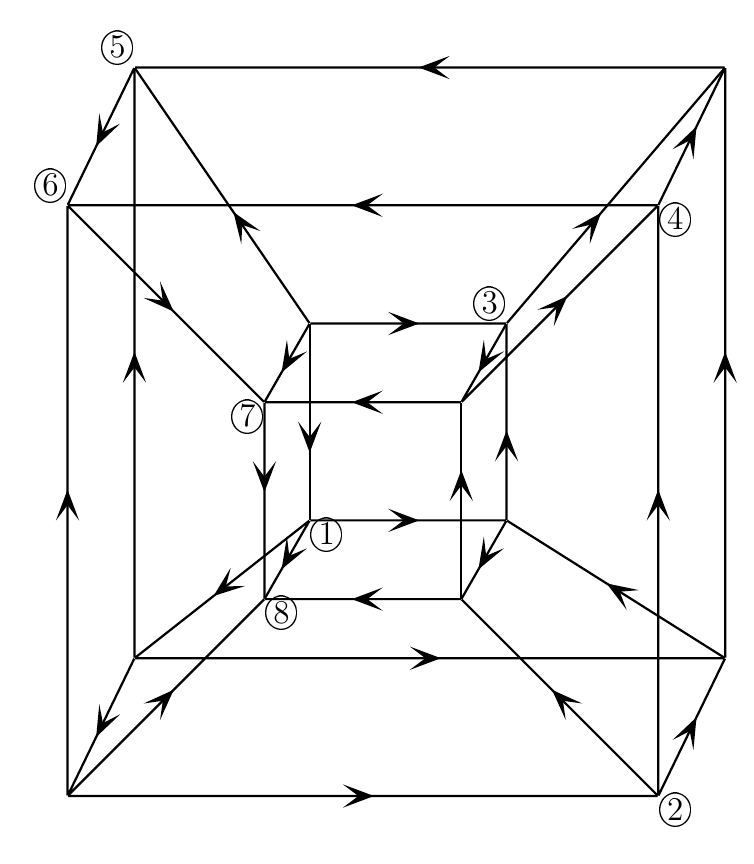
\begin{tikzpicture}[scale=2.5]
    

\pgfarrowsdeclare{mytipnew}{mytipnew} 
{ 
  \arrowsize=0.2pt 
  \advance\arrowsize by .5\pgflinewidth 
  \pgfarrowsleftextend{-4\arrowsize-2\pgflinewidth} 
  \pgfarrowsrightextend{2\pgflinewidth} 
} 
{ 
  \arrowsize=1pt 
  \advance\arrowsize by .5\pgflinewidth 
  \pgfsetdash{}{0pt} % do not dash 
  \pgfsetroundjoin   % fix join 
  \pgfsetroundcap    % fix cap 
  \pgfpathmoveto{\pgfpoint{-4\arrowsize}{3\arrowsize}}
  \pgfpathlineto{\pgfpoint{4\arrowsize}{0\arrowsize}}
  \pgfpathlineto{\pgfpoint{-4\arrowsize}{-3\arrowsize}}
  \pgfpathlineto{\pgfpoint{0\arrowsize}{0\arrowsize}}
  \pgfpathlineto{\pgfpoint{-4\arrowsize}{3\arrowsize}}
%   \pgfusepathqstroke 
  \pgfusepathqfill
}
 \tikzset{
  % style to apply some styles to each segment of a path
  every node/.style={draw,circle,inner sep=0pt,minimum size=0pt},
  on each segment/.style={
     decorate,
     decoration={
      show path construction,
      moveto code={},
      lineto code={
         \path [#1]
         (\tikzinputsegmentfirst) -- (\tikzinputsegmentlast);
      },
      curveto code={
         \path [#1] (\tikzinputsegmentfirst)
         .. controls
         (\tikzinputsegmentsupporta) and (\tikzinputsegmentsupportb)
         ..
         (\tikzinputsegmentlast);
      },
      closepath code={
         \path [#1]
         (\tikzinputsegmentfirst) -- (\tikzinputsegmentlast);
      },
     },
  },
  mid arrow/.style={postaction={decorate,decoration={
         markings,
         mark=at position .5 with {{\arrow[#1]{mytipnew}}},
      }}},
  near arrow/.style={postaction={decorate,decoration={
         markings,
         mark=at position .4 with {{\arrow[#1]{mytipnew}}},
      }}},
  far arrow/.style={postaction={decorate,decoration={
         markings,
         mark=at position .6 with {{\arrow[#1]{mytipnew}}},
      }}},
 }


\tikzstyle{edge} = [draw,thick,postaction={on each segment={mid arrow=black}},black]
\tikzstyle{edgefar} = [draw,thick,postaction={on each segment={far arrow=black}},black]
\tikzstyle{edgenear} = [draw,thick,postaction={on each segment={near arrow=black}},black]
\newcommand{\mycircle}[1]{\large{\raisebox{.5pt}{\textcircled{\raisebox{-.9pt} {#1}}}}}
\path(0,0) node[label=below right:{\mycircle{8}}] (v0) {}
     (0,1) node (v1)[label=below left:\mycircle{7}] {}
     (1,0) node (v2) {}
     (1,1) node (v3) {}
     (0.23, 0.4) node (v4)[label=below right:\mycircle{1}] {}
     (0.23,1.4) node (v5) {}
     (1.23,0.4) node (v6) {}
     (1.23,1.4) node (v7)[label=above left:\mycircle{3}] {}
     (-1,-1) node (v8) {}
     (-1,2) node (v9)[label=above left:\mycircle{6}] {}
     (-0.66,2.7) node (v13)[label=above left:\mycircle{5}] {}
     (-0.66,-0.3) node (v12) {}
     (2,-1) node (v10)[label=below right:\mycircle{2}] {}
     (2.34,-0.3) node (v14) {}
     (2,2) node (v11)[label=below right:\mycircle{4}] {}
     (2.34,2.7) node (v15) {};
% \node[above of=v1,node distance=0.2in] (v1l) {2};
\draw[edge]
%  (v1) -- (v0)
 (v2) -- (v0)
%  (v2) -- (v3)
 (v3) -- (v1)
 (v3) -- (v11)
 (v4) -- (v0)
 (v4) -- (v6)
 (v4) -- (v12)
 (v5) -- (v1)
%  (v5) -- (v4)
 (v5) -- (v7)
%  (v5) -- (v13)
 (v6) -- (v2)
%  (v6) -- (v7)
 (v7) -- (v3)
%  (v7) -- (v15)
 (v8) -- (v0)
 (v8) -- (v9)
 (v8) -- (v10)
 (v9) -- (v1)
 (v10) -- (v2)
 (v10) -- (v11)
 (v10) -- (v14)
 (v11) -- (v9)
 (v11) -- (v15)
 (v12) -- (v8)
 (v12) -- (v13)
 (v12) -- (v14)
 (v13) -- (v9)
 (v14) -- (v6)
 (v14) -- (v15)
 (v15) -- (v13);
 \draw[edgenear] (v5) -- (v13) (v7) -- (v15) (v1) -- (v0) (v6) -- (v7);
 \draw[edgefar] (v2) -- (v3) (v5) -- (v4);
    %  \draw[edge] (v1) -- (v0);
    %  \draw[edge] (v2) -- (v0);
    %  \draw[edge] (v2) -- (v3);
    %  \draw[edge] (v3) -- (v1);
    %  \draw[edge] (v3) -- (v11);
    %  \draw[edge] (v4) -- (v0);
    %  \draw[edge] (v4) -- (v6);
    %  \draw[edge] (v4) -- (v12);
    %  \draw[edge] (v5) -- (v1);
    %  \draw[edge] (v5) -- (v4);
    %  \draw[edge] (v5) -- (v7);
    %  \draw[edge] (v5) -- (v13);
    %  \draw[edge] (v6) -- (v2);
    %  \draw[edge] (v6) -- (v7);
    %  \draw[edge] (v7) -- (v3);
    %  \draw[edge] (v7) -- (v15);
    %  \draw[edge] (v8) -- (v0);
    %  \draw[edge] (v8) -- (v9);
    %  \draw[edge] (v8) -- (v10);
    %  \draw[edge] (v9) -- (v1);
    %  \draw[edge] (v10) -- (v2);
    %  \draw[edge] (v10) -- (v11);
    %  \draw[edge] (v10) -- (v14);
    %  \draw[edge] (v11) -- (v9);
    %  \draw[edge] (v11) -- (v15);
    %  \draw[edge] (v12) -- (v8);
    %  \draw[edge] (v12) -- (v13);
    %  \draw[edge] (v12) -- (v14);
    %  \draw[edge] (v13) -- (v9);
    %  \draw[edge] (v14) -- (v6);
    %  \draw[edge] (v14) -- (v15);
    %  \draw[edge] (v15) -- (v13);
    %  \draw[selected edge] (v4) -- (v10);
    %  \draw[selected edge] (v10) -- (v7);
    %  \draw[selected edge] (v7) -- (v11);
    %  \draw[selected edge] (v11) -- (v13);
    %  \draw[selected edge] (v13) -- (v9);
    %  \draw[selected edge] (v9) -- (v1);
    %  \draw[selected edge] (v1) -- (v0);
 \end{tikzpicture}
 }
 \caption{The only 4-AUSO (up to an isomorphism) on which HPI performs $8$ vertex evaluations. The $8$ vertices are numbered in sequence. This AUSO does not satisfy the Holt-Klee conditions. Notice, for example, that the inner $3$-AUSO does not have $3$ vertex-disjoint paths from source to sink.}
 \label{fig:4auso-8hpi}
\end{figure}


%\newpage

\section{Proofs from Section 5}
\label{app:lowerbound}
\setcounter{theorem}{9}

We provide a proof of Theorem~\ref{thm:lowerbound}, which uses the MDP designed by Melekopoglou and Condon~\shortcite{Melekopoglou+Condon:1994}, shown in Figure~\ref{fig:mnc-mdp}. Recall from Section~\ref{sec:lowerbound} that we only consider states $s \in \{1, 2, \dots, n\}$ as a part of our analysis.

For this proof, we find it convenient to consider a slight modification to RPI. If a policy $\pi$ has $m > 1$ improvable states, note that RPI obtains $\pi^{\prime} \succ \pi$ by picking uniformly at random among the $2^{m} - 1$ improving policies in $I(\pi)$. We consider an algorithm RPI1 that instead picks $\pi^{\prime}$ uniformly at random from $I(\pi) \cup \{\pi\}$. The reason for so doing is that RPI1 can be implemented by independently switching each improvable state with probability $1/2$, which simplifies our analysis. The consequence, though, is that RPI1 is not strictly a PI algorithm, since with a finite probability, we can get $\pi^{\prime} = \pi$. This probability is at most $1/2$, and therefore, the expected number of policies visited by RPI1 (which might contain repetitions) is at most twice the expected number of policies visited by RPI. To prove the theorem, we show below that the former quantity is at least $n + 1$.

Building on  Melekopoglou and Condon~\shortcite{Melekopoglou+Condon:1994}, first we obtain a simple rule to check if a state $s$ is switchable. 


\begin{lemma}
\label{l1}
For a policy $\pi$ for $M_n$, a state $s$ is switchable if and only if $$\sum_{s'\le s}\pi(s) \equiv 0 \mod 2.$$
\end{lemma}

\begin{proof}
%\textit{Definition 2.1} in 
For states $s \in \{1, 2, \dots, n\}$, Melekopoglou and Condon~\shortcite{Melekopoglou+Condon:1994} define
%$a(k)$ for every 
$$a(1)=-\frac{1}{2}
\text{ and }
a(s+1)=a(s)\left(\frac{1}{2}-\pi(s) \right).$$
It is easy to verify from the definition
%from \textit{Corollary 2.3} in 
that 
%$$a(s+1)=\frac{(-1)^{\sum_{s'\le s}\pi(s)}}{2^s}a(1)=\frac{(-1)^{\sum_{s'\le s}\pi(s)}}{2^s}\frac{-1}{2}$$
%Thus, 
$a(s+1)$ is negative if and only if $\sum_{s'\le s}\pi(s) \equiv 0 \mod 2$
~\cite[see Corollary 2.3]{Melekopoglou+Condon:1994}.
Since $a(s+1)=a(s)(\frac{1}{2}-\pi(s))$, $a(s+1)$ is negative if and only if $\pi(s)=0$ and $a(s)<0$, or $\pi(s)=1$ and $a(s)>0$. Based on the structure of $M_{n}$, Melekopoglou and Condon\shortcite[see Corollary 2.4]{Melekopoglou+Condon:1994} show that the latter condition is equivalent to $s$ being switchable.
%dynamics o This latter event Combined with \textit{Corollary 2.4} in \shortcite[see Corollary 2.4]{Melekopoglou+Condon:1994}, the proof is complete.
% Proof follows from \textit{Corollary 2.3} and \textit{Corollary 2.4} in \cite{mnv}. Vertex $k$ is switchable if and only if 
% For $k=1$, $a(1)=-\frac{1}{2}$ is negative and hence vertex $1$ is switchable if and only if $S_1$ is $0$. Assume the statement holds for all positive integers $k' \le k$. Since $a(k+1)=a(k)(\frac{1}{2}-S_k)$, if $S_k$ is $0$ and $a(k)$ is negative, or $S_k$ is $1$ and $a(k)$ is positive, $a(k+1)$ is negative. If vertex $k$ is switchable 
\end{proof}

The crucial step in our proof is to define a \textit{progress} function $f$ on the policy space, which is then shown to be non-increasing with respect to PI updates. 

\begin{definition}
\label{d2}
    For a policy $\pi$ for $M_n$, $$f(\pi) \mathrel{\overset{\makebox[0pt]{\mbox{\normalfont\tiny\sffamily def}}}{=}} \min \left(\textsf{states}(T^\pi) \cup \{n+1\}\right).$$
\end{definition}
In other words, $f(\pi)$ is defined to be the smallest switchable state if $\pi$ is not optimal, and $n + 1$ if it is $\pi^{\star}$. The lemma below establishes the monotonicity of $f$.
%, $f(\pi^{*}) \mathrel{\overset{\makebox[0pt]{\mbox{\normalfont\tiny\sffamily def}}}{=}} n+1$.
\begin{lemma}
\label{l3}
    If RPI1 visits the policies $\pi^0, \pi^1, \dots, \pi^m$ in sequence, then for $1\le i \le m$, $f(\pi^{i-1})\le f(\pi^i)$.
\end{lemma}

\begin{proof}
Since we stop when there are no improvable states, $f(\pi^{m-1}) \leq f(\pi^m)=n+1$. Otherwise assume that $i<m$. Let $f(\pi^{i-1}) = s$. Since vertex $s$ is the smallest switchable state in $\pi^{i-1}$, any state $s'$ will not be switched in $\pi^{i-1}$ for $1\le s' < s$, and hence $\pi^i(s')=\pi^{i-1}(s')$.
% \textcolor{red}{From Lemma~\ref{l1}, we have $\sum_{s''\le s}\pi^{i-1}(s'') \equiv 1 \mod 2$ for $1 \le s' < s$. This implies $\pi$ is of the form $10^{s-2}1w$ for some $w \in \{0,1\}^{n-s}$ if $s\ge 2$ or $0w^{\prime}$ for some $w^{\prime}\in\{0,1\}^{n-1}$ if $s=1$. WHILE THIS RED PORTION MIGHT BE TRUE, IS IT ACTUALLY USED TO OBTAIN THE NEXT STATEMENT? ALSO I ASSUME THE $\pi$ IN THIS PORTION IS $\pi^{i - 1}$. YES?}
% Since states $1, 2, \dots, s-1$ are not switchable for $\pi^{i-1}$, we have $\pi^i(s')=\pi^{i-1}(s')$ for $1 \le s' < s$.
It follows from  Lemma~\ref{l1} that states $1, 2, \dots, s-1$ are not switchable in $\pi^i$. Thus, $f(\pi^i)\ge s = f(\pi^{i-1})$.
\end{proof}

% \begin{corollary}
%     For policies $\pi$ and $\pi^{\prime}$ for $M_{n}$, if $\pi^{\prime} \succeq \pi$, then $f(\pi) \le f(\pi')$.
% \end{corollary}

% \begin{proof}
% 4. EXPLAIN THIS PART--WHY SUCH A PI ALGORITHM EXISTS. ACTUALLY DO YOU USE THIS COROLLARY? IT DOESN'T SEEM TO BE CORRECT---COMPARE, FOR EXAMPLE, POLICIES 010 AND 111 IN FIGURE 1. ONE DOMINATES THE OTHER, BUT THERE'S NO PATH. THE RESULT IS TRUE IF THE DOMINATING ONE IS AN OPTIMAL POLICY. REMOVE THE COROLLARY IF IT IS NOT USED. - Not Used, but corollary is valid for MDP being considered.

% We have a policy iteration algorithm that visits the policies $\pi^0,\pi^1,...,\pi^m$ where $\pi^0=\pi$ and $\pi^m=\pi'$, where the switching rule is to only switch improvable states where the policy differs from $\pi'$. Applying Lemma \ref{l3} gives us the above result.
% \end{proof}

Next we show that as RPI1 proceeds, with sufficiently high probability $f$ increases quite slowly. It follows thereafter that at least $n + 1$ policy evaluations must be made in expectation if $\pi^{0} = 0^{n}$ is the initial policy ($f(\pi^{0})$ and $f(\pi^{\star})$ differ by $n$).

%the expected number of RPI updates to drop this potential function from $f(\pi^0)$ to $f(\pi^{\star})$ is at least $n+1$ if we choose $\pi^0(s)=0$ for all $s \in \{1, 2, \dots, n\}$. %Sometimes we will represent a policy $\pi$ as a bit-string $w_1w_2{\dots}w_n \in \{0,1\}^n$ where $\pi(s)=w_s$. In this notation, $\pi^0 = 0^n$ and $\pi^{\star} = 10^{n-1}$. 


\begin{lemma}
\label{l4}
    If RPI1 visits the policies $\pi^0, \pi^1, \dots, \pi^m$ in sequence, then for $1\le i \le m$, $t\ge 0$, $$\mathbb{P}\{f(\pi^{i}) - f(\pi^{i-1}) \ge t\} \le \frac{1}{2^t}.$$
\end{lemma}


\begin{proof}
%We first provide a high level overview. If $f(\pi^{i-1})=s$, the event $E=\{f(\pi^{i})\ge s+t\}$, requires $1,2,...,s+t-1$ not to be switchable in $\pi^i$. This in turn, due to Lemma~\ref{l1}, requires some of the randomly made decisions in switching states of $\pi^{i-1}$ to turn out in a particular way favourable to $E$. Since states $1,2,...,s-1$ were not switchable and remain same in $\pi^{i-1}$ and $\pi^i$, there is no decision to be made at these states. Only the decisions made at states $s, s+1,...,s+t-1$ need to be favourable to $E$. This happens with probability $\frac{1}{2^t}$. For some $\pi^{i-1}\in \Pi, t\in \mathbb{N}$, $f(\pi^{i})\ge s+t$ might not be possible at all (for example, when $t>n$), in which case the left hand side of the inequality is $0\le \frac{1}{2^t}$. Now we provide the formal argument. Let $[x]$ denote the set $\{1, 2, \dots, x\}.$


%If $t=0$, the inequality follows directly from Lemma~\ref{l3}. Henceforth we assume $t>0$.
If $t=0$, the RHS is 1 and the result trivial. Henceforth we assume $t > 0$. The proof splits into cases $f(\pi^{i - 1}) = 1$ and $f(\pi^{i - 1}) > 1$, which we consider in turn. 
Let $[x]$ denote the set $\{1, 2, \dots, x\}.$

If $f(\pi^{i-1})=1$, $s=1$ is switchable in $\pi^{i-1}$. From Lemma~\ref{l1}, $\pi^{i-1}(1)=0$. Thus, let $\pi^{i-1}=0^{s^\prime}x$ for some $1 \le s^\prime \le n$, $x\in \{0,1\}^{n-s^\prime}$, and $x$ starts with $1$ or $x$ is empty. Applying Lemma~\ref{l1} for states $1,2,\dots,s'+1$, we get that states $1,2,\dots,s'$ are switchable in $\pi^{i-1}$ and $s'+1$ is not switchable in $\pi^{i-1}$, if $s'+1\in [n]$. If $f(\pi^{i})\ge t+1$, the states $1,2,\dots,t$ are not switchable in $\pi^i$. Applying Lemma~\ref{l1} for states $1,2,\dots,t$, we get that $\pi^{i}=10^{t-1}y$ where $y\in \{0,1\}^{n-t}$. If $s'=n$, $t\le n=s'$. $t$ cannot be greater than $s^\prime$ if $s'+1\in [n]$ as that will imply $\pi^{i}(s^\prime+1)=0\ne \pi^{i-1}(s^\prime+1)$, despite $s^\prime+1$ not being switchable in $\pi^{i-1}$. Hence, if $t > s'$, $\mathbb{P}\{f(\pi^i)\ge t+1\}=0\le \frac{1}{2^t}$. Otherwise $t \le s'$. Therefore, states $1,2,\dots,t$ are switchable in $\pi^{i-1}$. To get to $\pi^i$ from $\pi^{i-1}$, the state $1$ must be switched and the states $2,3, \dots,t$ must not be switched. As each state is switched with probability $\frac{1}{2}$ by RPI1, the probability of this event happening is exactly $\frac{1}{2^t}$.

If $f(\pi^{i-1})=s>1$, $s$ is switchable in $\pi^{i-1}$ and $1,2,\dots,s-1$ are not switchable in $\pi^{i-1}$. Applying Lemma~\ref{l1} for states $1,2,\dots,s$, we get $\pi^{i-1}=10^{s-2}10^{s'}x$ for some $0 \le s^\prime \le n-s$, $x\in \{0,1\}^{n-s-s^\prime}$, and $x$ starts with $1$ or $x$ is empty. Applying Lemma~\ref{l1} for states $s+1,s+2,\dots,s+s'$, we get that states $s+1,s+2,\dots,s+s'$ are also switchable in $\pi^{i-1}$ and $s+s'+1$ is not switchable in $\pi^{i-1}$, if $s+s'+1\in [n]$. Note that since $i-1<m$, $\pi^{i-1}\ne \pi^{*}$ and hence $s\le n$. If $f(\pi^{i})\ge s+t$, the states $1,2,\dots,s+t-1$ are not switchable in $\pi^i$. Applying Lemma~\ref{l1} for states $1,2,\dots,s+t-1$, we get that $\pi^{i}=10^{s+t-2}y$ where $y\in \{0,1\}^{n-s-t+1}$. If $s+s'=n$, $s+t-1\le n=s+s'$. $s+t-1$ cannot be greater than $s+s'$ if $s+s'+1\in [n]$ as that will imply $\pi^{i}(s+s'+1)=0\ne \pi^{i-1}(s+s'+1)$, despite $s+s'+1$ not being switchable in $\pi^{i-1}$. Hence, if $s+t-1 > s+s'$, $\mathbb{P}\{f(\pi^i)\ge s+t\}=0\le \frac{1}{2^t}$. Otherwise $s+t-1 \le s+s'$. Therefore, states $s,s+1,\dots,s+t-1$ are switchable in $\pi^{i-1}$. To get to $\pi^i$ from $\pi^{i-1}$, the state $s$ must be switched and the states $s+1,s + 2, \dots,s+t-1$ must not be switched. As each state is switched with probability $\frac{1}{2}$ by RPI1, the probability of this event happening is exactly $\frac{1}{2^t}$.
% Assume $f(\pi^{i-1}) = s$. Let $s'>s$ be the vertex with the smallest index after $s$ which is not switchable. If all vertices after $s$ are switchable, we let $s'=n+1$.Using Lemma \ref{l1}, $\pi^{i-1}(s'')=0$ for $s < s'' < s'$ and $\pi^{i-1}(s')=1$ if $s' \le n$. Since $s'$ is not switched, $\pi^i(s')=\pi^{i-1}(s')=1$ and hence either $s'$ or $s'-1$ should be switchable in $\pi^i$. So $f(\pi^i)\le s'$.
% \newline
% For $f(\pi^{i-1}) < f(\pi^i)$, $s$ should not be switchable in $\pi^i$. Since states less than $s$ are not switched, and whether or not $s$ is switchable in $\pi^i$ depends on the states $1, 2,...,s$, $s$ must have been switched in $\pi^{i-1}$. This happens with probability $\frac{1}{2}$. So $Pr[f(\pi^{i}) - f(\pi^{i-1}) \ge 1] \le \frac{1}{2}$.
% \newline
% For $f(\pi^i)=s+t$ where $t < s'-s$, we require $s+t$ to be switchable in $\pi^i$, $s''$ to be not switchable in $\pi^i$ for $s \le s'' < s+t$. For this states $s$ and $s+t$ must have been switched in $\pi^{i-1}$ and $s+t'$ must not be switched for $ 1 \le t' < t$. Since each switchable state is switched independently with probability $\frac{1}{2}$, the probability of this event is $\frac{1}{2^{t+1}}$. Thus $Pr[f(\pi^{i}) - f(\pi^{i-1}) = t] = \frac{1}{2^{t+1}}$ for $t < s'-s$. So $Pr[f(\pi^{i}) - f(\pi^{i-1}) \ge t] = \sum_{t'=t}^{t'=s'-s-1}Pr[f(\pi^{i}) - f(\pi^{i-1}) = t']=\sum_{t'=t}^{t'=s'-s-1}\frac{1}{2^{t'+1}} \le \frac{1}{2^t}$.
\end{proof}

%\textcolor{red}{In the definition and the theorem be more precise. (1) It seems like $N(i)$ must be defined as a MINIMUM over all policies $\pi$  with $f(\pi) = i$. (2) Use $\pi$ instead of of $\pi^{0}$ in the definition. (3) Is this proof by induction? Add a few more lines to make it more clear---induction on which variable? (4) Iterations/Evaluations etc. can be off-by-1 when we're counting. If you begin with $\pi^{\star}$, do you use 0 iterations ot 1 iteration? Be precise with this wording in both definition and theorem. (5) Also, why is the denominator $2^{t + 1}$ in the recursion for $N(s)$ rather than $2^{t}?$ Explain in words in the proof itself.}

\begin{definition}
    We define $L:\Pi\to \mathbb{R}_{\ge 0}$, where $L(\pi)$ is the expected number of policies evaluated by RPI1 starting from $\pi$.
\end{definition}
Note that even if we start from $\pi^0=\pi^{*}$, we need to evaluate $\pi^0$ to know that it is optimal. Hence $L(\pi^{*})=1$.
\begin{definition}
    We define $N:[n+1]\to \mathbb{R}_{\ge 0}$, where $$N(s) = \min_{\pi\in\Pi, f(\pi)= s} L(\pi).$$
\end{definition}
It directly follows from the definition that $N(f(\pi))\le L(\pi)$ for any $\pi\in\Pi$.
\begin{theorem}
	For $s\in [n+1]$, $N(s) \ge n+2-s$.
\end{theorem}
\begin{proof}
If $s=n+1$, $f(\pi)= n+1$ is true only for $\pi=\pi^*$. Hence $N(n+1)=L(\pi^{*})=1\ge n+2-(n+1)$.

Now, let $s\in [n]$. Let $\pi$ be a policy such that $N(s)=L(\pi)$. Hence $f(\pi)=s$. Since $f(\pi^{*})=n+1$, $\pi$ is not optimal. Let $\pi^{\prime}$ be obtained from $\pi$ by an RPI1 update.

First we upper-bound the expectation of $f(\pi^\prime)$. Since $f(\pi')$ is a non-negatively valued random variable, we can use the following expression for its expectation. 
\begin{align*}
\mathbb{E}[f(\pi^\prime)] &= \sum_{n+1 \ge s^\prime \ge 1}\mathbb{P}\{f(\pi^\prime)\ge s'\} 
\\ &= \sum_{s\ge s^\prime \ge 1}1 + \sum_{n+1 \ge s^\prime > s}\mathbb{P}\{f(\pi^\prime)\ge s'\}\\
&\le s + \sum_{n+1 \ge s^\prime > s}\frac{1}{2^{s^\prime-s}}\\
&\le s + \sum_{k=1}^{\infty}\frac{1}{2^{k}}\\
&= s+1.
\end{align*}
Now, assuming inductively that $N(s^\prime)\ge n+2-s^\prime$ for $s< s^\prime\le n+1$, we can lower-bound $N(s)=L(\pi)$ as
\begin{align*}
N(s) &=&& 1+\sum_{\pi^{\prime\prime}\in\Pi}L(\pi^{\prime\prime})\mathbb{P}\{\pi^{\prime}=\pi^{\prime\prime}\}
\\ &\ge&& 1+\sum_{\pi^{\prime\prime}\in\Pi}N(f(\pi^{\prime\prime}))\mathbb{P}\{\pi^{\prime}=\pi^{\prime\prime}\}
\\ &=&& 1+\sum_{n+1 \ge s^\prime \ge 1} \Bigg[ \sum_{\pi^{\prime\prime}\in\Pi, f(\pi^{\prime\prime})=s^\prime}N(s^\prime)\mathbb{P}\{\pi^{\prime}=\pi^{\prime\prime}\}\Bigg] 
\\ &=&& 1+\sum_{n+1 \ge s^\prime \ge 1}N(s^\prime)\Bigg[\sum_{\pi^{\prime\prime}\in\Pi, f(\pi^{\prime\prime})=s^\prime}\mathbb{P}\{\pi^{\prime}=\pi^{\prime\prime}\}\Bigg]
\\ &=&& 1+\sum_{n+1 \ge s^\prime \ge 1}N(s^\prime)\mathbb{P}\{f(\pi^{\prime})=s^\prime\}
\\ &=&& 1+\sum_{n+1 \ge s^\prime \ge s}N(s^\prime)\mathbb{P}\{f(\pi^{\prime})=s^\prime\},
% \\ & && (\because \mathbb{P}(f(\pi^{\prime})<s)=0)
% \\
\end{align*}
%\begin{flushright}
%$(\because %\mathbb{P}(f(\pi^{%\prime})<s=f(\pi))%=0)$.
%\end{flushright}
since $\mathbb{P}\{f(\pi^{\prime})<s=f(\pi)\}=0$. We rearrange terms in a convenient form, and apply $\mathbb{E}[f(\pi^{\prime})] \leq s+ 1$, to get
\begin{align*}
N(s)&\ge&& 1+\sum_{n+1 \ge s^\prime \ge s}(N(s^\prime)-n-2+s')\mathbb{P}\{f(\pi^{\prime}\}=s^\prime\}
\\
&&&+\sum_{n+1 \ge s^\prime \ge s}(n+2-s')\mathbb{P}\{f(\pi^{\prime})=s^\prime\}
\\
% &\text{\textcolor{red}{Don't get the next two steps}}\\
&=&& 1+\sum_{n+1 \ge s^\prime \ge s}(N(s^\prime)-n-2+s')\mathbb{P}\{f(\pi^{\prime}\}=s^\prime\}
\\
&&&+n+2-\sum_{n+1 \ge s^\prime \ge s}s'\mathbb{P}\{f(\pi^{\prime}\}=s^\prime\}
\\
&=&& \sum_{n+1 \ge s^\prime \ge s}(N(s^\prime)-n-2+s')\mathbb{P}\{f(\pi^{\prime})=s^\prime\}
\\
&&&+n+3-\mathbb{E}[f(\pi')]
\\
&\ge && \sum_{n+1 \ge s^\prime \ge s}(N(s^\prime)-n-2+s')\mathbb{P}\{f(\pi^{\prime})=s^\prime\}
\\
&&&+n+2-s.
% \\
% &\text{\textcolor{red}{Because induction hypothesis}}\\
% &\ge n+3 +(N(s)-n-2+s)\mathbb{P}(f(\pi^{\prime})=s)
%         \\ &- \sum_{n+1 \ge s^\prime \ge s}s^\prime\mathbb{P}(f(\pi^{\prime})=s^\prime)
% \\ &\ge n+3+\frac{N(s)-n-2+s}{2}-\mathbb{E}[f(\pi^\prime)]
% \\ &\ge n+2-s+\frac{N(s)-n-2+s}{2}.
% \\ &\ge 1+\sum_{n+1 \ge s^\prime \ge s}N(s^\prime)(\mathbb{P}(f(\pi^{\prime})\ge s^\prime)-\mathbb{P}(f(\pi^{\prime})\ge s^\prime+1)
% \\ &= 1 + N(s)\mathbb{P}(f(\pi^\prime)\ge s) \\ &+ \sum_{n+1 \ge s^\prime > s}\mathbb{P}(f(\pi^\prime)\ge s)(N(s^\prime)-N(s^\prime-1))
\end{align*}
By the induction hypothesis, $N(s')-n-2+s^{\prime}$ is non-negative for $s^{\prime}>s$. Therefore, after removing terms corresponding to $s^{\prime}>s$, we get $$ N(s) \ge n+2-s+(N(s)-n-2+s)\mathbb{P}\{f(\pi')=s\},$$ which rearranges into $$(N(s)-n-2+s)(1-\mathbb{P}\{f(\pi')=s\})\ge 0 .$$
% \end{align*}

Now, $\mathbb{P}\{f(\pi')=s\}$ cannot be $1$ because there is a policy $\pi''=\textsf{modify}(\pi, \{(s, a)\}) \in \Pi$, where $a\in \{0,1\}$ and $a\ne\pi(s)$, such that $\mathbb{P}\{\pi'=\pi''\}>0$ and $f(\pi'')>s$ (since $s$ is not switchable in $\pi''$). Hence, we must have
$N(s) \ge n+2-s$.
\end{proof}

At this point, Theorem~\ref{thm:lowerbound} follows as a corollary; the statement of the theorem is reproduced below.

\begin{corollary}
	Starting from $\pi^0=0^n$, the expected number of policies RPI evaluates on $M_n$ before terminating is at least $\frac{n+1}{2}$.
    % $N(n+1) = 0$. $N(i) \ge n+2-i$ for $1 \le i \le n$.
\end{corollary}

\begin{proof}
% If $f(\pi^0)=n+1$, $\pi^0=\pi^{*}$ is already optimal and RPI halts.
% \newline
% If 
% If $f(\pi^{i-1})=s$, Lemma \ref{l4} shows that $Pr[f(\pi^i)\ge s+t] \le \frac{1}{2^t}$. Hence $N(s) \ge 1+\sum_{t=0}^{n+1-s}\frac{N(s+t)}{2^{t+1}}=1+\sum_{t=0}^{n-s}\frac{N(s+t)}{2^{t+1}}$. For $s=n$, we have $N(s)=2$. Assume $N(s')\ge n+2-s'$ for $n \ge s'>s$. Thus $N(s) \ge 1+\frac{N(s)}{2}+\sum_{t=1}^{n+1-s}\frac{n+2-s-t}{2^{t+1}} \ge 1+\frac{N(s)}{2}+\sum_{t=1}^{\infty}\frac{n+2-s-t}{2^{t+1}} = 1 + \frac{N(s)+n-s}{2}$. Thus $N(s) \ge n+2-s$.
For $\pi^0=0^{n}$, $f(\pi^0)=1$. Thus 
\begin{equation*}
L(\pi^0)\ge N(1)\ge n+2-1=n+1.
\end{equation*}
In other words, RPI1 evaluates at least $n + 1$ policies in expectation, which implies RPI evaluates at least half that number of policies in expectation.
\end{proof}

\end{appendices}


\end{document}
